\documentclass[letterpaper,fontsize=9pt,DIV=12]{scrartcl}
% \documentclass[a4paper,10pt,DIV=14]{scrartcl}
% \documentclass[a4paper,10pt,DIV=13]{scrartcl} % scrreprt

\usepackage[utf8]{inputenc}
\setlength{\parskip}{0.8em}
\setlength{\parindent}{0pt}

% ######################################################################################################################
%         Custom Packages
% ######################################################################################################################

\usepackage{graphicx}
\usepackage[table,dvipsnames]{xcolor}

\graphicspath{{figures/fst_plot_pdf/}}

\usepackage[square,sort,comma,numbers]{natbib}
\usepackage[english]{babel}
\usepackage[notlot,nottoc,numbib]{tocbibind}
\renewcommand{\bibsection}{\section{References}}
\AtBeginDocument{\def\bibname{References}}

% https://tex.stackexchange.com/questions/267675/pdftex-error-pdflatex-file-ecbx0800-font-ecbx0800-at-600-not-found
\usepackage{lmodern}

% https://reu.dimacs.rutgers.edu/Symbols.pdf
\usepackage{amssymb}

% https://tex.stackexchange.com/a/6105
% \usepackage[binary-units=true]{siunitx}
\usepackage{siunitx}

% https://tex.stackexchange.com/questions/94845/problems-with-toprule-and-midrule-in-a-table
\usepackage{booktabs}

% https://ctan.org/pkg/relsize
\usepackage{relsize}

\usepackage[bf,format=plain]{caption}

% https://tex.stackexchange.com/questions/135358/changing-the-formatting-of-subcaption-for-reference
\usepackage[labelformat=simple]{subcaption}
\renewcommand\thesubfigure{(\alph{subfigure})}

% https://tex.stackexchange.com/a/39981
\usepackage[nolist,nohyperlinks]{acronym}

% http://bytesizebio.net/2013/03/11/adding-supplementary-tables-and-figures-in-latex/
\newcommand{\beginsupplement}{%
    \setcounter{table}{0}
    \renewcommand{\thetable}{\arabic{table}}%
    \setcounter{figure}{0}
    \renewcommand{\thefigure}{\arabic{figure}}%
}
%     \renewcommand{\thetable}{S\arabic{table}}%
%     \renewcommand{\thefigure}{S\arabic{figure}}%

\usepackage{amsmath}
\usepackage{xfrac}
\usepackage{bm}
\usepackage{scalerel,stackengine}

% Increase row spacing in align envs
% https://tex.stackexchange.com/a/14680/171851
\addtolength{\jot}{0.75em}

% Excluded the following lines from the pnas class file.
% Include them here again to ensure correct setup.
% See https://tex.stackexchange.com/q/1863
\usepackage[colorlinks=true, allcolors=blue]{hyperref}
% \renewcommand\UrlFont{\color{black}\sffamily}
\urlstyle{rm}

% https://tex.stackexchange.com/a/78020
\pdfsuppresswarningpagegroup=1

% \externaldocument[main:]{main}

% \usepackage{nameref,zref-xr}
% \zxrsetup{toltxlabel}
% \zexternaldocument*{pppp}

% https://tex.stackexchange.com/questions/180019/grouping-two-tables-one-above-the-other
\usepackage{hypcap} % fix the links

% https://tex.stackexchange.com/questions/109467/footnote-in-tabular-environment
\usepackage{threeparttable}
% \usepackage[flushleft]{threeparttable}

% Sections with dots in TOC
% https://tex.stackexchange.com/a/53901/171851
\usepackage{tocloft}
\renewcommand{\cftsecleader}{\cftdotfill{\cftdotsep}}

% LEFT-ALIGN THE AUTHOR LIST
% Overleaf syntax highlighting gets messed up by this, but it works.
% Commented out now to not mess with overleaf for now.
% https://tex.stackexchange.com/a/364432/171851
% \usepackage{xpatch}
% \makeatletter
% \xpatchcmd{\@maketitle}{\begin{center}}{\begin{flushleft}}{}{}
% \xpatchcmd{\@maketitle}{\end{center}}{\end{flushleft}}{}{}
% \xpatchcmd{\@maketitle}{\begin{tabular}[t]{c}}{\begin{tabular}[t]{@{}l@{}}}{}{}
% \makeatother

% ######################################################################################################################
%         Custom Commands
% ######################################################################################################################

% Preparation for the todo command
\newcounter{todo}
\setcounter{todo}{0}
\newcounter{popoolissue}
\setcounter{popoolissue}{0}

% ----------------------------------------------------------
% TODO command:

% Use the first line below to show them,
% use the second to hide them,
% and comment out the respective other line.
% LaTeX is so easy ;-)

% \newcommand\todo[1]{{\stepcounter{todo}\color{purple}{TODO \arabic{todo}: #1}}}
\newcommand\todo[1]{}

% Same for "popoolissue", which we use to annotate our questions for the popoolation team
% \newcommand\popoolissue[1]{{\stepcounter{popoolissue}\color{purple}{ITEM \arabic{popoolissue}: #1}}}
\newcommand\popoolissue[1]{}
% ----------------------------------------------------------


% todo environment
% \newcounter{todo}
% \newcommand\todo[1]{\refstepcounter{todo}{\color{purple}{#1}}\addcontentsline{todolist}{subsection}{\thetodo:~#1}}
% un-comment the next line in order to hide all todos:
% \renewcommand\todo[1]{}
% \newcommand\moi[1]{{\color{orange}{#1}}}

% Suppress KOMA script warning
% https://tex.stackexchange.com/q/412368
\DeclareOldFontCommand{\bf}{\normalfont\bfseries}{\mathbf}

\newcommand\citeay[1]{\citeauthor{#1} (\citeyear{#1}) \cite{#1}}
\usepackage{cleveref}

% https://nw360.blogspot.de/2007/12/rename-bibliography-title-in-latex.html
% https://tex.stackexchange.com/a/306268
% \renewcommand\refname{References}
% \renewcommand\bibname{References}
% \addto{\captionsenglish}{%
%   \renewcommand{\bibname}{References}
% }

% Define custom styles
\newcommand\toolname{\textsc}
\newcommand\taxonname{\textit}
\newcommand\formatname{\texttt}
\newcommand\langname{\texttt}

% \newcommand\figref[1]{Figure~\ref{#1}}
% \newcommand\tabref[1]{Table~\ref{#1}}
% \newcommand\eqnref[1]{Equation~(\ref{#1})}

\newcommand\figref[1]{Figure~\ref{#1}}
\newcommand\tabref[1]{Table~\ref{#1}}
\newcommand\eqnref[1]{Eq.~(\ref{#1})}
\newcommand\secref[1]{Section~\ref{#1}}

\newcommand{\samplesize}{n}
\newcommand{\coverage}{c}
\newcommand{\empfreq}{\widehat{f}}
\newcommand{\thetapi}{\widehat{\theta_\pi}}
\newcommand{\watterson}{\widehat{\theta_\text{W}}}
\newcommand{\fst}{F\textsubscript{ST}}
\newcommand{\mathfst}{F_\text{ST}}
\newcommand{\neifst}{F_\text{ST}^\text{Nei}}
\newcommand{\hudsonfst}{F_\text{ST}^\text{Hudson}}
\newcommand{\neiestimator}{\widehat{F}_\text{ST}^\text{Nei}}
\newcommand{\hudsonestimator}{\widehat{F}_\text{ST}^\text{Hudson}}
\newcommand{\eg}{e.\,g.,~}
\newcommand{\ie}{i.\,e.,~}

% Seq error extensions by Jeff
\usepackage{xr}
\usepackage{times}
\usepackage{slantsc}
\usepackage{amsthm}
\usepackage{xspace}
\newtheorem*{cor}{Corollary}
\newtheorem{theorem}{Theorem}

% Seq error extensions by Jeff
\newcommand\iid{\mathrel{\stackrel{\makebox[0pt]{\mbox{\normalfont\tiny i.i.d.}}}{\sim}}}
\newcommand*{\piw}{$\pi_\text{within}$\xspace}
\def\mathpiw{\pi_\text{within}}
\newcommand*{\pib}{$\pi_\text{between}$\xspace}
\def\mathpib{\pi_\text{between}}
\newcommand*{\pit}{$\pi_\text{total}$\xspace}
\def\mathpit{\pi_\text{total}}

% \def\subsubsec#1{\noindent\textbf{#1.}}
% \def\sepop#1{s^{(#1)}}

% https://tex.stackexchange.com/questions/103408/symbol-for-corresponds-to-equals-sign-with-hat
\newcommand\equalhat{%
\let\savearraystretch\arraystretch
\renewcommand\arraystretch{0.3}
\begin{array}{c}
\stretchto{
    \scalerel*[\widthof{=}]{\wedge}
    {\rule{1ex}{3ex}}%
}{0.5ex}\\
=%
\end{array}
\let\arraystretch\savearraystretch
}

% ######################################################################################################################
%         Title and Header
% ######################################################################################################################

% ORCID
\newbox{\orcidlogo}
\sbox{\orcidlogo}{\large
\includegraphics[height=1.8ex]{figures/logo-orcid.pdf}}
\newcommand{\orcid}[1]{\href{https://orcid.org/#1}{\usebox{\orcidlogo}\,}}

\addtokomafont{title}{\raggedright}
\addtokomafont{author}{\raggedright\setlength{\tabcolsep}{0pt}}
\addtokomafont{date}{\raggedright}

% Title Page
\title{Pool-Sequencing corrections for population genetic statistics}
% \subtitle{Genesis and Gappa: Library and Toolkit for \\Working with Phylogenetic (Placement) Data.}
\author{\orcid{0000-0002-1340-9644}Lucas Czech\textsuperscript{a,*}, \orcid{0000-0002-3199-1447}Jeffrey P. Spence\textsuperscript{b}, and \orcid{0000-0001-5711-0700}Moisés Expósito-Alonso\textsuperscript{a,c,d,*}}
\date{}

% ######################################################################################################################
%         Document
% ######################################################################################################################

\begin{document}

% \begin{abstract}
% abstract...
% \end{abstract}

% \beginsupplement
% \maketitle

\begingroup
\let\center\flushleft
\let\endcenter\endflushleft
\maketitle
\endgroup
\vspace*{-3.5em}
% Correspondence: 
% \href{mailto:moisesexpositoalonso@gmail.com}{moisesexpositoalonso@gmail.com},
% \href{mailto:luc@s-cze.ch}{luc@s-cze.ch}
\textsuperscript{a}{Department of Plant Biology, Carnegie Institution for Science, Stanford, USA.\\}
\textsuperscript{b}{Department of Genetics, Stanford University, Stanford, USA.\\}
\textsuperscript{c}{Department of Biology, Stanford University, Stanford, USA.\\}
\textsuperscript{d}{Department of Global Ecology, Carnegie Institution for Science, Stanford, USA.\\}
\textsuperscript{*}{To whom correspondence should be addressed: \href{mailto:lczech@carnegiescience.edu}{\color{black}{lczech@carnegiescience.edu}},
% \href{mailto:jspence@stanford.edu}{\color{black}{jspence@stanford.edu}}, 
and \href{mailto:moisesexpositoalonso@gmail.com}{\color{black}{moisesexpositoalonso@gmail.com}}}

% Custom title, as the template is a bit broken...
% \makeatletter
% {\LARGE \textbf{\@title}}
% It was written by \@author\space on \@date

% ######################################################################################################################
%         Supplement Text
% ######################################################################################################################

% \section*{Overview}
% \label{supp:sec:SoftwareComparison}

\vspace*{2em}
% \\
\setlength{\fboxsep}{2em}
\fbox{%
  \parbox{48em}{
        \large
        \textbf{Version: 2023-09-12}
        \\ \\
        The latest version of this document can be found at %\\
        \url{https://github.com/lczech/pool-seq-pop-gen-stats}
        \\
        When citing this document or equations in it, %\\
        we recommend to also mention the version, as section and equation numbering might change.
  }%
}
\vspace*{2em}

\section*{Abstract}
\label{supp:sec:Abstract}

This document describes our assessment of the specific pool-sequencing (Pool-seq) equations for population genetic measures of diversity (such as $\theta_\pi$, $\theta_\text{Watterson}$, Tajima's $D$), and differentiation (such as $\mathfst$).
The aim of these equations is to correct for the noises of pool sequencing, specifically limited sample size (number of individuals pooled, or pool size~$\samplesize$) and limited coverage (number of reads obtained from those individuals, or coverage $\coverage$).

We re-render some approaches originally presented and implemented in \toolname{PoPoolation} \cite{Kofler2011a} and \toolname{PoPoolation2} \cite{Kofler2011b}, as well as other publications.  We re-derive estimators of genetic diversity, and suggest some improvements that fix standing issues when working with Pool-seq data. Furthermore, we (re-)derive two consistent (asymptotically unbiased) estimators for \fst{} for pool sequencing data, using two distinct definitions of \fst{}, that correct for both sources of noise mentioned above.  We also evaluate the different estimators for \fst{} here using simulated data, showing their particular biases.  Lastly, we derive novel estimators for \fst{} that additionally take sequencing error into account.  

Our main findings are as follows. (1) Correcting for Pool-seq noise in Tajima's D in order to obtain results that are numerically comparable to values obtained from individual sequencing is difficult, and the approach of \toolname{PoPoolation} has statistical shortcomings. We hence recommend not interpreting their values of Tajima's D quantitatively, and instead compare $\theta_{\pi}$ and $\theta_{w}$ directly without Pool-seq corrections. (2) Some of the established Pool-seq estimators for \fst{} are biased upward for small pool sizes and low read depth; we hence recommend using the estimators presented here instead.

The estimators presented here are implemented in our tool 
%\href{https://github.com/lczech/grenedalf}{grenedalf}.
grenedalf: \url{https://github.com/lczech/grenedalf}


% ======================================================================================================
%          TOC
% ======================================================================================================

\pagebreak

\tableofcontents

\vspace*{5em}
\textbf{Note on sources:}
\begin{itemize}
    \item This document is partially based on the PoPoolation equations document \texttt{correction\_equations.pdf} as found in their code repository; we provide a copy at \url{https://github.com/lczech/popoolation/blob/master/files/correction_equations.pdf}. This document derives some of the equations implemented, but also contains equations that are not implemented in \toolname{PoPoolation} but may be of interest for a deeper understanding of the topic.
    \item Furthermore, we incorporated several implementation details from the reverse-engineered code of \toolname{PoPoolation} and \toolname{PoPoolation2}. We want this document to represent the equations that are actually computed when running these programs (and their re-implementations in \toolname{grenedalf}), as we feel that they need a more thorough assessment than what is available in the current literature.
    \item Lastly, for the avid reader, apart from these documents and the original publications of \toolname{PoPoolation} \cite{Kofler2011a} and \toolname{PoPoolation2} \cite{Kofler2011b}, we also recommend the \toolname{npstat} \cite{Ferretti2013} and \toolname{poolfstat} \cite{Hivert2018,Gautier2022-zd} publications, which contain further renderings of some of the equations.
\end{itemize}

\pagebreak

% ======================================================================================================
%          Definitions
% ======================================================================================================

\section{Preliminaries}
\label{supp:sec:Definitions}

% We here assume basic familiarity with pool sequencing concepts.
% Please refer to \citeay{Kofler2011a} for details on pool sequencing data and its biases.
% \todo{maybe we should cite some more sources here?}

% ------------------------------------------------------------------------------------------------------
%          Pool Sequencing
% ------------------------------------------------------------------------------------------------------

\subsection{Pool Sequencing Data and Notation}
\label{supp:sec:Definitions:sub:PoolSequencing}

We first define the input that we assume to be given for all subsequent equations.
In the software implementation of the equations, these are based on the input data, or set by the user as parameters.

$\samplesize$ :
Pool size, as given in the dataset (and in the software, provided by the user). This is the number of individuals (haplotypes) that were pooled together for the sequencing of a population. Note on the pool size for different levels of ploidy:  The pool sequencing approach assumes the pool size to be the number of distinct haplotypes in the population that have been sampled. Hence, for instance for 100 diploid individuals, the number of haplotypes (and hence the pool size) is 200.

$\coverage$ :
Observed coverage. This is the number of reads sequenced from the pool that span a focal position in the genome. 
% \todo{this being a sum of Cs, isn't that also a random variable, and should be captialized?  Yes and no -- throughout we assume that it is not random, which is fine -- the randomness in the coverage is ancillary (\url{https://en.wikipedia.org/wiki/Ancillary_statistic}) to the estimation of the frequencies, and so in some sense it's uninteresting / unimportant whether it's random or not.}

$b$ :
Minimum allele count, provided by the user.
We do not want to consider SNPs with fewer than $b$ alternative reads in the data, as they might be sequencing errors.
Note that we assume $b$ to be a user-provided constant,
and hence leave it out of (most) function arguments for simplicity.

For most equations we will consider a single pool sequencing sample (one population, or one experiment), but in cases where we consider multiple samples (multiple pool-sequenced populations), we will denote the different samples with subscripts in parentheses, such as $\samplesize_{(1)}, \samplesize_{(2)},\ldots$ or $\coverage_{(1)}, \coverage_{(2)}, \ldots$ to denote different populations or experiments.

Beyond these data-specific and user-specified parameters, we will use the following notation.  In general, we will use capital letters for random variables in our model of pool sequencing, which will be described shortly in \secref{supp:sec:model}.  We will also differentiate sample quantities (\ie those that are computed from data) from their population counterparts (\ie parameters that describe the population from which the data were sampled) with hats.  For example, we differentiate the frequency of the $A$ allele in the whole population, $f_A$, from the empirical frequency of $A$ nucleotides in our pool sequencing sample, $\empfreq_A$.

$\tau$ :
Index over nucleotides, with $\tau \in \left\{ \text{A}, \text{C}, \text{G}, \text{T} \right\}$ being implicit in any summations.

$C_\tau$ :
Nucleotide counts, \ie how many reads have a certain nucleotide $\tau$ at a given position in the genome. Note that we generally do not make assumptions about the focal position in the genome being biallelic, unless stated otherwise.

$\coverage = \sum_\tau C_\tau$ : The (total) coverage at a given position.

$f_\tau$ :
Nucleotide frequencies in the population, \ie the proportion of haplotypes that have nucleotide $\tau$ at the focal position.

$\empfreq_\tau$ :
Empirical nucleotide frequencies, \ie $\empfreq_\tau := C_\tau / \coverage$. Naturally, $\sum_\tau \empfreq_\tau = 1$.
%\sfrac{c_\tau}{C}$

% $p$, $q$ :
% For biallelic SNP positions, we simplify and instead of the four $f_\tau$ values,
% just use $p$ for the frequency of the reference allele, and $q$ for the frequency of the alternative allele.

$m$ :
Index of summation over potential levels of coverage $\coverage$.

$k$ :
Index of summation over potential pool sizes $\samplesize$.

% $a$: (generalized) harmonic numbers

% $h$ : heterozygosity

% ------------------------------------------------------------------------------------------------------
%          Harmonic Numbers
% ------------------------------------------------------------------------------------------------------

We will also make use of the generalized harmonic numbers, which frequently arise in coalescent theory.  Define $a_1$ and $a_2$ as the sum of (squared) reciprocals of the first $n$ positive integers:
%
\begin{align}
    \label{eq:an}
    a_1(n) &:= \sum_{k=1}^{m} \frac{1}{k}
    \\
    \label{eq:bn}
    a_2(n) &:= \sum_{k=1}^{m} \frac{1}{k^2}
\end{align}
%


We use this notation as a compromise between Equation (3.6) of \citeay{Hahn2018} and the notation of $a_n$ and $b_n$ used in \citeay{Achaz2008} for these quantities.

\subsection{Statistical Model of Pool Sequencing}
\label{supp:sec:model}

We consider a simple model of pool sequencing as a series of multinomial samplings from a population.  In particular we assume the following model, where $N_\tau$ is the (unobserved) number of individuals in the pool with the $\tau$ allele:

\begin{align*}
(N_A, N_C, N_G, N_T) &\sim \text{Multinomial}\left(\samplesize, (f_A, f_C, f_G, f_T)\right)\\
(C_A, C_C, C_G, C_T) | (N_A, N_C, N_G, N_T) &\sim \text{Multinomial}\left(\coverage, \left(\frac{N_A}{\samplesize}, \frac{N_C}{\samplesize},\frac{N_G}{\samplesize},\frac{N_T}{\samplesize}\right)\right)
\end{align*}

Throughout, we will repeatedly make use of the following results:
\begin{align}
\mathbb{E}\left[\empfreq_\tau\right] = f_\tau, \label{eq:frequnbiased}
\end{align}
and
\begin{align}
\mathbb{E}\left[\left(\frac{\coverage}{\coverage-1}\right)\left(\frac{\samplesize}{\samplesize-1}\right)\left(1-\sum_\tau\empfreq_\tau^2\right)\right] = 1-\sum_\tau f_\tau^2. \label{eq:hetunbiased}
\end{align}

To see Equation~\ref{eq:frequnbiased} we can use the tower property:
\[
\mathbb{E}\left[\empfreq_\tau\right] = \mathbb{E}\left[\mathbb{E}\left[\empfreq_\tau \mid N_\tau \right]\right] = \mathbb{E}\left[\frac{N_\tau}{n}\right] = f_\tau.
\]
To obtain Equation~\ref{eq:hetunbiased}, we make use of the following fact about binomial distributions.  Suppose $X$ is binomially distributed with parameters $m$ and $p$, then $X$ can be represented as the sum of $m$ independent, identically distributed Bernoulli random variables, $Y_1,\ldots,Y_m$ that take the value $1$ with probability $p$ and $0$ with probability $1-p$.  We can then see:
\begin{align*}
\mathbb{E}\left[X(m-X)\right] &= \mathbb{E}\left[\sum_{i=1}^m\sum_{j=1}^mY_i(1-Y_j)\right]\\
&= m\mathbb{E}\left[Y_1(1-Y_1)\right] + m(m-1)\mathbb{E}\left[Y_1(1-Y_2)\right]
\end{align*}
where the second equality follows from the linearity of expectation and the fact that all of the $Y_i$s are identically distributed.  Then, since $Y_i$ is either $0$ or $1$, $Y_i(1-Y_i)$ must be zero.  Finally, by independence,
\[
\mathbb{E}\left[Y_1(1-Y_2)\right] = \mathbb{E}\left[Y_1\right]\left(1-\mathbb{E}\left[Y_2\right]\right) = p(1-p).
\]
Therefore,
\[
\mathbb{E}\left[X(m-X)\right]  = m(m-1)p(1-p)
\]

We can now make use of this result twice along with the tower property to obtain Equation~\ref{eq:hetunbiased}:
\begin{align*}
\mathbb{E}\left[\left(\frac{\coverage}{\coverage-1}\right)\left(\frac{\samplesize}{\samplesize-1}\right)\left(1-\sum_\tau\empfreq_\tau^2\right)\right] &= \sum_\tau\left(\frac{\coverage}{\coverage-1}\right)\left(\frac{\samplesize}{\samplesize-1}\right) \mathbb{E}\left[\empfreq_\tau(1-\empfreq_\tau)\right]\\
&=  \sum_\tau\left(\frac{\coverage}{\coverage-1}\right)\left(\frac{\samplesize}{\samplesize-1}\right) \left(\frac{1}{\coverage^2}\right) \mathbb{E}\left[C_\tau\left(c-C_\tau\right)\right]\\
&= \sum_\tau\left(\frac{1}{\coverage(\coverage-1)}\right)\left(\frac{\samplesize}{\samplesize-1}\right) \mathbb{E}\left[\mathbb{E}\left[C_\tau\left(c-C_\tau\right) \mid N_\tau\right]\right]\\
&= \sum_\tau\left(\frac{\samplesize}{\samplesize-1}\right) \mathbb{E}\left[\frac{N_\tau}{\samplesize}\left(1-\frac{N_\tau}{\samplesize}\right)\right]\\
&= \sum_\tau\frac{1}{\samplesize(\samplesize-1)}\mathbb{E}\left[N_\tau\left(\samplesize - N_\tau\right)\right]\\
&= \sum_\tau f_\tau(1-f_\tau) = 1 - \sum_\tau f_\tau^2.
\end{align*}

The last equality holds as $\sum_\tau f_\tau = 1$.

% ======================================================================================================
%          Theta Pi
% ======================================================================================================

\section{Pairwise Heterozygosity \texorpdfstring{$\theta_\pi$}{Theta Pi}}
\label{supp:sec:ThetaPi}

First, we derive estimators for the pairwise heterozygosity, $\theta_\pi$, also called Tajima's $\pi$.  Formally, pairwise heterozygosity is the probability that two haploids drawn \emph{from the population} have different alleles at a position chosen uniformly at random.  We always assume that the population is large so that for a particular site, $\theta_\pi = 1 -\sum_\tau f_\tau^2$, which can be seen by noting that the probability that we pick two individuals with the $\tau$ allele is $f_\tau^2$.

If we were to sequence individuals, it would be straightforward to derive unbiased estimators for $\theta_\pi$, but instead we obtain a pool of reads, which introduces two major issues.  The first is that we no longer have access to individuals.  If we had sequenced individuals, we could estimate $\theta_\pi$ by looking at two individuals and asking if they have different alleles at a position, but in pool sequencing, we can only look at two different reads and ask if they have different alleles.  The issue is that we cannot know whether those reads were from the same individual or from different individuals, so a naive estimator of $\theta_\pi$ that just looks at pairwise differences between reads will be biased because in some fraction of times those reads will have come from the same individual, and hence must have the same allele (ignoring sequencing error).  The second major issue is that positions where only a small number of reads have a particular allele could be an artifact of sequencing error.  As such, PoPoolation restricts to sites where there are either exactly $0$ or at least $b$ reads supporting each allele.

Below we derive PoPoolation's estimator of pairwise heterozygosity, $\thetapi$, which addresses both of the issues listed above.  Dealing with the bias from pool-sequencing is straightforward.  Restricting to positions where there are at least $b$ reads with the minor allele is more complex, however, and requires additional assumptions that will almost certainly not be met in practice.  In particular, the $\thetapi$ estimator crucially relies on the assumption that the population is evolving neutrally and is at equilibrium -- in technical terms, the derivation relies on the sample frequency spectrum being proportional to $1/k$, which is to say that the probability that $k$ out of $\samplesize$ individuals have the derived allele at a segregating site has probability proportional to $1/k$.  In practice, natural selection, gene flow, or fluctuations in effective population size can all cause deviations from this assumption, and these deviations will result in $\thetapi$ being a biased estimator of $\theta_\pi$.

% ------------------------------------------------------------------------------------------------------
%          Unbiased Pool-seq estimator
% ------------------------------------------------------------------------------------------------------

% \subsection{Unbiased Pool-seq estimator of \texorpdfstring{$\theta_{\pi}$}{Theta Pi} for biallelic SNPs}
% \label{supp:sec:ThetaPi:sub:PoolSequencing}

\subsubsection*{PoPoolation Pool-seq estimator, \texorpdfstring{$\thetapi$}{Theta Pi hat}}
\label{supp:sec:ThetaPi:sub:PoolSequencing}

% % ------------------------------------------------------------------------------------------------------
% %     Definition for biallelic SNPs
% % ------------------------------------------------------------------------------------------------------
%
% \subsubsection*{Definition for biallelic SNPs}
% \label{supp:sec:ThetaPi:sub:PoolSequencing:sub:BasicDefinition}

PoPoolation begins by defining %
\begin{align}
    \label{eq:ThetaPiFreq2}
    \thetapi^{\samplesize\to\infty} &:= \frac{\coverage}{\coverage-1} \left(1 - \sum_\tau \empfreq_\tau^2 \right),
\end{align}
%
which is equal to the left hand side of Equation~\ref{eq:hetunbiased} up to a factor of $\frac{\samplesize}{\samplesize-1}$.  This indicates that this is a biased estimator of the heterozygosity at this site, but the bias is on the order of $O\left(\frac{1}{\samplesize}\right)$, which means that PoPoolation assumes an extremely large pool size, which is why we use the $\samplesize\to\infty$ superscript.

At this point, the PoPoolation equations document begins to simplify the above equation, and then breaks it down for biallelic SNPs. However, their (and our) implementation differs from this, and uses the above equation that works with any (not just biallelic) SNPs. We hence do not introduce these simplifications here.
% \todo{I thought a bit more about this. the heterozygosity is indeed computed from all four bases. BUT: the below equations are still assuming biallelic SNPs! is that a problem?! it's solvable by just using biallelic snps as in the computation -- but what would it mean theoretically to use this correction for non-biallelic snps?  JPS: their whole correction assumes that the mutation rate is vanishingly small so that you should (almost) never see non-biallelic SNPs.  In practice, I would think that multi-allelic SNPs would actually be quite rare and so shouldn't be something we worry about too much.}
Note however that the computation is still only conducted on biallelic sites, as the correction term introduced below assumes this. This means, we are assuming that multiallelic sites are rare, which is true for small mutation rates.

\popoolissue{We think that it is makes sense to compute only on biallelic SNPs, as this is a theoretical derivation of $4N_e\mu$, which assumes the infinitesimal model (which does not allow for multi-allelic loci). Still, we briefly wanted to check in with you here. Our guess is that the computation in code is just done for all four nucleotides to keep the code simple -- but the function only gets called for biallelic sites, so it behaves as if it was only computed for biallelic SNPs. Is that right?}

% \todo{(Moi) I think it is fine that below it assumes biallelic SNPs. It is a theoretical derivation of 4Neu, one of which assumptions is the infinitesimal model (a mutation is unlikely to happen two times in the same place, so multiallelic loci are assumed impossible). JPS: yes! exactly!}

% ------------------------------------------------------------------------------------------------------
%    Expected value of population mutation rate $\theta$ from nucleotide diversity
% ------------------------------------------------------------------------------------------------------

\subsubsection*{Bias of $\thetapi^{\samplesize\to\infty}$ when restricting to sites with at least $b$ minor allele reads}
\label{supp:sec:ThetaPi:sub:PoolSequencing:sub:ExpectedValue}

Other than the bias from the finite pool size, $\thetapi^{\samplesize\to\infty}$ is a reasonable estimator of the pairwise heterozygosity at a given site.  To obtain an overall estimate of $\theta_\pi$, we could average $\thetapi^{\samplesize\to\infty}$ across all sites.  PoPoolation seeks to avoid including sites that appear to be segregating solely because of sequencing error, however, which adds a complication.  We expect that sequencing errors should be rare, and so it would be extremely unlikely to see $b$ or more reads supporting a particular allele solely due to sequencing error.  As such, we can remove all sites with fewer than $b$ reads supporting the minor allele.  This is problematic, however, and biases the estimator --- while removing such sites certainly removes most or all sites that are segregating solely due to sequencing error, it also removes a large number of sites where the mutation just happens to be at low frequency.

The approach that PoPoolation takes is to assume neutrality and an equilibrium demography (all variation is neutral, and the population is of constant size and in mutation-drift equilibrium), calculate the bias of $\thetapi^{\samplesize\to\infty}$, and introduce a term to correct for that bias.  Despite using sequencing error as a motivation, PoPoolation ignores sequencing error in the following derivation.  The derivation will assume biallelic sites, and all expectations in this section will be with respect to both the randomness in the Pool-Seq experiment as well as the randomness in the evolutionary process.  

To begin, we compute the expectation of $\thetapi^{\samplesize\to\infty}$ when we treat sites with fewer than $b$ reads supporting the minor allele as not contributing to $\thetapi^{\samplesize\to\infty}$.  Since we are assuming that we are only looking at biallelic sites, we will use $M$ to denote the number of reads supporting the derived allele.  Letting $\mathcal{E}_b$ be the event that at least $b$ reads support the minor allele, we see
%
\begin{align}
\mathbb{E}\left[\thetapi^{\samplesize\to\infty} \mathbb{I}\left\{\mathcal{E}_b\right\}\right] &= \sum_{m=b}^{\coverage-b} \mathbb{E}\left[\thetapi^{\samplesize\to\infty} \mid M=m \right] \mathbb{P}(M = m)\\
&= \mathbb{P}\left(\text{Site is a SNP}\right)\sum_{m=b}^{\coverage-b} \mathbb{E}\left[\thetapi^{\samplesize\to\infty} \mid M=m \right] \mathbb{P}\left(M = m \mid \text{Site is a SNP}\right)\\
&=  2\mathbb{P}\left(\text{Site is a SNP}\right)\sum_{m=b}^{\coverage-b} \frac{m(\coverage-m)}{\coverage(\coverage-1)} \mathbb{P}\left(M = m \mid \text{Site is a SNP}\right)
\label{eq:ExpectationThetaPi}
% \mathbb{E}(\theta_\pi|C) &= P(\mbox{SNP} | n) \cdot \sum_{m=b}^{C-b} \frac{2m (C-m)}{C(C-1)} \cdot P(m|C,n)
% \\
% &= P(\mbox{SNP} | n) \cdot \frac{2}{C(C-1)} \cdot \sum_{m=b}^{C-b} m(C-m) \cdot P(m|C,n)
\end{align}
%
In words, the expected value is computed by summing all possible SNP counts (that exceed the minimum count $b$) that can occur in a pool with coverage $\coverage$, weighted by the probability to have each of those counts.  As we are using the derived allele count $m$ in the equation above, and either the derived or ancestral allele could be the minor allele, we ``sandwich'' our potential values for the coverage between $b$ and $\coverage-b$.

The two probabilities used above are computed as follows.

$\mathbb{P}\left(\text{Site is a SNP}\right)$ is the probability of observing a SNP in our pool of $\samplesize$ individuals.  Here we invoke our neutrality and equilibrium assumptions, where a classical result from coalescent theory gives:
%
\begin{align}
\label{eq:PSNP}
\mathbb{P}\left(\text{Site is a SNP}\right) = 1- \prod_{k=1}^{\samplesize-1} \frac{1}{1+\frac{\theta_\pi}{k}} \approx \theta_\pi a_1(n-1)
\end{align}

where the final approximation ignores terms on the order of  $\theta_\pi^2$, which implicitly assumes that the mutation rate is small.

$\mathbb{P}\left(M = m \mid \text{ Site is a SNP }\right)$ is the probability of observing $m$ as the derived allele count in a SNP with $\coverage$ reads from a pool of $n$ individuals.  We can further break this down by conditioning on the number of individuals in the pool that have the derived allele, which we will call $\widetilde{M}$:
%
\begin{align}
    \label{eq:Pmcn}
    \mathbb{P}\left(M = m \mid \text{site is a SNP}\right) &= \sum_{k=1}^{n-1} \mathbb{P}\left(M=m \mid \widetilde{M} = k\right)\mathbb{P} \left( \widetilde{M} = k \mid \text{site is a SNP}\right)\\
    %&= \sum_{k=1}^{n-1} P(m|C,n,k) \frac{1/k}{\sum_{j=1}^{n-1} 1/j} \\
    &= \frac{1}{a_1(n-1)}  \sum_{k=1}^{n-1} \frac{1}{k}  \mathbb{P}\left(M=m \mid\widetilde{M} = k\right)
\end{align}
where the second line follows from another classic result in coalescent theory that (assuming neutrality, equilibrium, and that $\theta_\pi$ is small) the probability that $k$ individuals in a pool of size $\samplesize$ have the derived allele given that a site is s SNP is $\frac{1}{ka_1(n-1)}$.

Finally, $ \mathbb{P}\left(M=m \mid \widetilde{M} = k\right)$ is the probability of having $m$ reads support the derived allele when $k$ individuals in the pool have the derived allele.  From our binomial sampling model of pool sequencing, this is:

%
\begin{align}
    \label{eq:Pmcnk}
     \mathbb{P}\left(M=m \mid \widetilde{M} = k\right) &= \binom{\coverage}{m} \left(\frac{k}{\samplesize}\right)^m \left(\frac{\samplesize-k}{\samplesize}\right)^{\coverage-m}
\end{align}
%
In words, this follows a binomial distribution, with $m$ successes out of $c$ trials
with a success probability of $k/n$ for each trial.
That is, we compute how likely it is to observe $m$ counts of the allele in $c$ reads,
given a frequency $k/n$ of that allele in the pool.
The count of the other allele is implicitly $c-m$.

Starting from \eqnref{eq:ExpectationThetaPi}, we can now put this together:
%
\begin{align}
\nonumber
\mathbb{E}\left[\thetapi^{\samplesize\to\infty} \mathbb{I}\left\{\mathcal{E}_b\right\}\right]  &=2\theta_\pi \sum_{m=b}^{\coverage-b} \frac{m(\coverage-m)}{\coverage(\coverage-1)} \sum_{k=1}^{n-1} \frac{1}{k} \binom{\coverage}{m} \left(\frac{k}{\samplesize}\right)^m \left(\frac{\samplesize-k}{\samplesize}\right)^{\coverage-m}
\end{align}

This shows that if we use our estimator $\thetapi^{\samplesize\to\infty}$ but treat as zero sites where the minor allele is not supported by at least $b$ reads, then the estimate will be biased by a factor of
\[
2\sum_{m=b}^{\coverage-b} \frac{m(\coverage-m)}{\coverage(\coverage-1)} \sum_{k=1}^{n-1} \frac{1}{k} \binom{\coverage}{m} \left(\frac{k}{\samplesize}\right)^m \left(\frac{\samplesize-k}{\samplesize}\right)^{\coverage-m}
\]

which we will now use to eliminate said bias.

%@\todo{Jeff, Lucas I think there is still something weird in the substitution of the P(SNP given n). As it is written using Theta= S/an, the substitution is not a probability but the number of segregating sites}


% ------------------------------------------------------------------------------------------------------
%     Final approximation for population mutation rate Theta
% ------------------------------------------------------------------------------------------------------

\subsubsection*{Unbiased estimate of $\theta_\pi$ when restricting to sites with at least $b$ minor allele reads}
\label{supp:sec:ThetaPi:sub:PoolSequencing:sub:FinalApprox}

Based on the previous section, we can construct an unbiased estimator for $\theta_\pi$ when restricting to sites with at least $b$ reads supporting the minor allele, which we denote by $\widehat{\theta}_{\pi,\text{pool}}$.  Let $\mathcal{S}_{bc}$ be the set of sites where the coverage is $c$, and at least $b$ reads support the minor allele, and let $\thetapi^{\samplesize\to\infty}(\ell)$ be the above estimator evaluated at the $\ell^\text{th}$ site (where above we suppressed the dependence on site because we only considered one site at a time).  Finally, let $\mathcal{C}$ denote the set of distinct observed coverage levels across the genome.  We then define  $\widehat{\theta}_{\pi,\text{pool}}$ as
%
\begin{align}
    \label{eq:ThetaPiPoolEstimate}
     \widehat{\theta}_{\pi,\text{pool}} &:= \frac{1}{\# \text{sites}} \cdot \sum_{c\in \mathcal{C}}
    \frac{
       \sum_{\ell \in \mathcal{S}_{bc}} \thetapi^{\samplesize\to\infty}(\ell)
    }{
        2\sum_{m=b}^{\coverage-b} \frac{m(\coverage-m)}{\coverage(\coverage-1)} \sum_{k=1}^{n-1} \frac{1}{k} \binom{\coverage}{m} \left(\frac{k}{\samplesize}\right)^m \left(\frac{\samplesize-k}{\samplesize}\right)^{\coverage-m}
%         \sum_{k=1}^{n-1} \frac{1}{k}  {C \choose m} \left(\frac{k}{n}\right)^m \left(\frac{n-k}{n}\right)^{C-m}
    }
\end{align}
%
% \todo{Hey Jeff, I think we need to change the above a bit. In the denominator, the coverage $c$ can be different per site, and hence needs to be evaluated at each site individually. Hence, in my original forumation of this, I just gave the equation for a single site, and then said that they are summed over all sites. Shall I change it back to that?  JPS: I changed this a bit. Let me know if it's unclear.  Basically we now do a weighted average over coverage levels and debias each coverage level appropriately.}

The approach to compute this for a window is to sum up all values across the SNPs in the window.
This is the equation as implemented in \toolname{PoPoolation} as the measure called \texttt{pi},
and implemented in our \toolname{grenedalf} as well. Note that the denominator only depends on the total coverage $\coverage$ and the pool size $\samplesize$, and hence only needs to be computed once per coverage level, yielding a significant computational speedup.

% \begin{align}
%  \mathbb{E}(\theta_\pi,c) = \theta a_1(n) \frac{C}{C-1}\sum_{m=b}^{C-b}\left( 1 -
% \left(\frac{m}{C}\right)^2 \right) \cdot \sum_{k=1}^{n-1} {C \choose m} \left(\frac{k}{n}\right)^m \left(\frac{n-k}{n}\right)^{C-m}  \frac{1}{k} \frac{1}{a_1(n)}
% \end{align}
%
% \begin{align}
% \mathbb{E}(\theta_\pi|C) &= P(\mbox{SNP} | n) \cdot \sum_{m=b}^{C-b} \frac{2m (C-m)}{C(C-1)} \cdot P(m|C,n)
% \\
% &= \theta \cdot a_1(n) \cdot \sum_{m=b}^{C-b} \frac{2m (C-m)}{C(C-1)} \cdot \frac{1}{a_1(n)} \sum_{k=1}^{n-1} \frac{1}{k} P(m|C,n,k) \\
% &= \theta \cdot a_1(n) \cdot \sum_{m=b}^{C-b} \frac{2m (C-m)}{C(C-1)} \cdot \frac{1}{a_1(n)} \sum_{k=1}^{n-1} \frac{1}{k} {C \choose m} \left(\frac{k}{n}\right)^m \left(\frac{n-k}{n}\right)^{C-m}
% \end{align}

% \clearpage

% ------------------------------------------------------------------------------------------------------
%          Computation in Windows
% ------------------------------------------------------------------------------------------------------

% \subsection{Computation in Windows}
% \label{supp:sec:ThetaPi:sub:Windows}

% not much to say here, so moved to above

% % ------------------------------------------------------------------------------------------------------
% %          Simplified Theta Pi
% % ------------------------------------------------------------------------------------------------------

% \subsection{Simplified Theta Pi}
% \label{supp:sec:ThetaPi:sub:Simplified}

% Not sure if needed.

% PoPoolation notes: also good for individual sequencing

% ======================================================================================================
%          Theta Watterson
% ======================================================================================================

\section{Watterson's Theta, \texorpdfstring{$\widehat{\theta}_w$}{}}
\label{supp:sec:ThetaWatterson}

% \todo{this section name has a hat, while the previous theta pi section name does not. Jeff, which one do you prefer? JPS: I prefer Hat for this section because Watterson's is explicitly an estimator, whereas $\theta_\pi$ as we defined it -- is a population-level parameter (i.e., the pairwise heterozygosity \emph{in the population})}

% \todo{JPS:  Hey Lucas -- I think that all of these should be divided by the number of SNPs, otherwise it's an estimate of the \emph{total} rate of mutation across all sites.  Just want to check that that's what's in the code...  --> it is! well, both, the absolute and relative value are printed. thanks for checking! dividing by the number of sites with sufficient coverage (according to the min count and min cov settings) to get the to relative one.}

% ------------------------------------------------------------------------------------------------------
%          Theta Watterson
% ------------------------------------------------------------------------------------------------------

% \subsection{Pool-Sequencing Correction}
% \label{supp:sec:ThetaWatterson:sub:PoolSequencing}

Under neutrality and equilibrium demography, $\theta_\pi$ is equal to $4N_e\mu =: \theta$, where $\theta$ is four times the effective population size $N_e$ times the per-generation mutation rate $\mu$, and hence, the estimator in the previous section can be used as an estimate of the population-scaled mutation rate.  An alternative estimate of the mutation rate is Watterson's theta, $\widehat{\theta}_w$, which is based on the number of segregating sites instead of the pairwise heterozygosity.  If we had sequenced $n$ individuals, the usual definition of $\widehat{\theta}_w$ is:
\[
\widehat{\theta}_w := \frac{S}{\text{\# sites} \cdot a_1(n-1) }
\]
where $S$ is the number of segregating sites; see e.\,g., Equation (3.5) of \citeay{Hahn2018}. In the pool sequencing case we might hope to just count up the number of sites that have more than one allele to use in place of $S$, but sequencing error is deeply problematic here.  Any place where any read has a sequencing error will look like a segregating site, vastly inflating our estimate of the true number of sites that are segregating in our sample.  PoPoolation therefore follows a similar approach as in the case of the pairwise heterozygosity, by only considering a site to be segregating if at least $b$ reads support each of two alleles.  Again, this restriction introduces bias, because it will miss many sites where one of the alleles really is at a low frequency --- but still segregating --- in the pool.  As before, we will compute this bias and then correct for it, again assuming neutrality, and equilibrium demography, and that the mutation rate is small enough to only focus on biallelic sites.


Formally, let $M_\ell$ be the number of reads supporting the derived allele at site $\ell$, and define
\begin{align}
%     \nonumber
    S_b(\ell) :=
    \begin{cases}
        1 & \text{if } b \le M_\ell \le \coverage-b
        \\
        0 & \text{otherwise}
    \end{cases}
\end{align}
%

We then define our naive Pool-Seq analog of Watterson's $\theta$ as
\[
\widehat{\theta}_w :=\frac{1}{\text{\# sites} \cdot a_1(\samplesize-1)}\sum_{\ell} S_b(\ell)
\]

Reasoning the same as above, we get the expected value of $\widehat{\theta}_w$ as
%
\begin{align}
    \nonumber
    \mathbb{E}\left[\widehat{\theta}_w\right]
    &= \frac{1}{a_1(\samplesize-1)} \cdot \mathbb{P}\left(\text{Site is a SNP}\right)
        \cdot \sum_{m=b}^{\coverage-b} \mathbb{P}\left(M = m \mid \text{Site is a SNP}\right)
    \\
    \intertext{
        with the two probability terms again as in \eqnref{eq:PSNP} and \eqnref{eq:Pmcn}, thus leading to
    }
    \label{eq:ExpectationThetaW}
    &= \frac{1}{a_1(n-1)} \cdot \theta\sum_{m=b}^{\coverage-b}\sum_{k=1}^{n-1} \frac{1}{k} \binom{\coverage}{m} \left(\frac{k}{\samplesize}\right)^m \left(\frac{\samplesize-k}{\samplesize}\right)^{\coverage-m}
\end{align}
%
To accommodate different coverage levels throughout the genome, denote the set of different coverage levels as $\mathcal{C}$, and the set of sites with coverage $c$ as $\mathcal{S}_c$. Equation~\ref{eq:ExpectationThetaW} immediately suggests the following unbiased estimator, which we denote $\widehat{\theta}_{w, \text{pool}}$:
%
\begin{align}
    \label{eq:CorrectedThetaEstimate}
    \widehat{\theta}_{w, \text{pool}} &:= \frac{1}{\text{\# sites}} \cdot \sum_{c \in \mathcal{C}}
    \frac{
        \sum_{\ell \in \mathcal{S}_c} S_b(\ell)
    }{
         \sum_{m=b}^{\coverage-b}\sum_{k=1}^{n-1} \frac{1}{k} \binom{\coverage}{m} \left(\frac{k}{\samplesize}\right)^m \left(\frac{\samplesize-k}{\samplesize}\right)^{\coverage-m}
    }
\end{align}

Again, the approach to compute this for a window is to sum up all values across the SNPs in the window.  As before, the denominator only depends on the coverage $\coverage$, and hence only needs to be computed once per coverage level that is present in the data.  This is the equation as implemented in \toolname{PoPoolation} as the measure called \texttt{theta}, and implemented in our \toolname{grenedalf} as well.

% ------------------------------------------------------------------------------------------------------
%          Simplified Theta Watterson
% ------------------------------------------------------------------------------------------------------

% \subsection{Simplified Theta Watteron}
% \label{supp:sec:ThetaWatterson:sub:Simplified}

% Not sure if needed.

% PoPoolation notes: also good for individual sequencing

% ======================================================================================================
%          Tajima's D
% ======================================================================================================

\section{Tajima's D}
\label{supp:sec:TajimaD}

{
\color{Maroon}
\setlength{\fboxsep}{2em}
\fbox{%
  \parbox{48em}{
        In the following, we describe our assessment of the pool-sequencing corrected equations for Tajima's D as presented in \toolname{PoPoolation}. We however find that their statistical approach has some shortcomings, as described below, and suspect that these significantly change the results. We hence recommend to \emph{not} use the correction terms, but instead use an uncorrected direct comparison of $\theta_\pi$ and $\theta_w$. This will not allow for a quantitative interpretation of the values in terms of the classical (non-pool) Tajima's D, but avoids biases of the statistics. See \secref{supp:sec:TajimaD:sub:RealDeal} for details. We still describe the equations here, for completeness, and elaborate on their issues below.
  }%
}
}

Above, we have defined pool-sequencing corrected estimators $\widehat{\theta}_{\pi,\text{pool}}$ and $ \widehat{\theta}_{w, \text{pool}}$.
Now, we want to use them to define a test akin to Tajima's D for pool sequencing.
We are here again following the PoPoolation approach, and re-derive their equations.

% ------------------------------------------------------------------------------------------------------
%          Pool-Sequencing Correction
% ------------------------------------------------------------------------------------------------------

\subsection{Pool-Sequencing Correction}
\label{supp:sec:TajimaD:sub:PoolSequencingCorrection}

The PoPoolation equations document derives the following estimator.
To the best of our knowledge, this is however not implemented in \toolname{PoPoolation};
instead, they compute Tajima's D as presented in the following \secref{supp:sec:TajimaD:sub:Classic}.
We still introduce the approach here, for reference, and in the hope that it might be helpful.

First, we define:
%
\begin{align}
    \widehat{d}_\text{pool} ~&:=~ \widehat{\theta}_{\pi,\text{pool}} ~-~ \widehat{\theta}_{w, \text{pool}}
\end{align}
%
and use this to define our statistic:
%
\begin{align}
    \label{eq:BasicTajimaD}
    D_\text{pool} ~&:=~ \frac{ \widehat{d}_\text{pool} }{ \sqrt{ \widehat{\text{Var}}( \widehat{d}_\text{pool}) }},
\end{align}
%
with a plug-in estimate of the variance of $ \widehat{d}_\text{pool}$.
To derive this plug-in estimate of the variance, we start with the standard expansion of the variance:
%
\begin{align}
    \nonumber
    \text{Var}( \widehat{d}_\text{pool} ) &= \mathbb{E}\left[ \widehat{d}_\text{pool}^2 \right] - \mathbb{E}\left[\widehat{d}_\text{pool}\right]^2
\end{align}
%
At this point, we use that $\mathbb{E}[\widehat{d}_\text{pool}] = 0$ (i.e., unbiased) for populations at equilibrium, since both $\widehat{\theta}_{\pi,\text{pool}}$ and $\widehat{\theta}_{w, \text{pool}}$ are unbiased estimates of $\theta$.  Therefore, $\mathbb{E}[\widehat{d}_\text{pool}]^2 = 0$.

Then, following PoPoolation, we compute the variance as:

\begin{align}
    \nonumber
    \text{Var}( \widehat{d}_\text{pool} ) &= \mathbb{E}( \widehat{d}_\text{pool}^2 )
    \\
    \nonumber
    &= \mathbb{P}\left(\text{Site is a SNP}\right) \sum_{m=b}^{c-b} \mathbb{E}\left[\widehat{d}_{\text{pool}}^2 \mid M=m \right] \cdot \mathbb{P}\left(M = m \mid \text{Site is a SNP}\right)
    \intertext{which can be resolved using equations \eqnref{eq:PSNP} and \eqnref{eq:Pmcn} from previous sections:}
    \label{eq:VarDPool}
    &= \theta \sum_{m=b}^{c-b}  \mathbb{E}\left[\left(\widehat{\theta}_{\pi,\text{pool}} -  \widehat{\theta}_{w,\text{pool}} \right)^2 \Big\vert\ M=m\right]    \cdot \sum_{k=1}^{n-1} \frac{1}{k}  \binom{c}{m} \left(\frac{k}{n}\right)^m \left(\frac{n-k}{n}\right)^{c-m}
\end{align}
%
Both $\widehat{\theta}_{\pi,\text{pool}}$ and $\widehat{\theta}_{w, \text{pool}}$ are completely determined once we fix $M$ to be $m$, so the only unknown quantity is $\theta$.
PoPoolation suggests using $\widehat{\theta}_{\pi,\text{pool}}$
on the same window on which we are computing $D_\text{pool}$, as our estimate of $\theta$ to obtain a plug-in estimate of the variance:
\[
\widehat{\text{Var}}( \widehat{d}_\text{pool} )  := \widehat{\theta}_{\pi, \text{pool}} \sum_{m=b}^{c-b} \mathbb{E}\left[\left(\widehat{\theta}_{\pi,\text{pool}} -  \widehat{\theta}_{w,\text{pool}} \right)^2 \Big\vert\ M=m\right]
    \cdot \sum_{k=1}^{n-1} \frac{1}{k}  \binom{c}{m} \left(\frac{k}{n}\right)^m \left(\frac{n-k}{n}\right)^{c-m}
\]

This assumes that all individuals contribute the same number of reads to the pool.
As stated above, both $\widehat{\theta}_{\pi,\text{pool}}$ and $\widehat{\theta}_{w, \text{pool}}$ are completely determined once we fix $M$ to be $m$, so these values can be pre-computed and stored to achieve a computational speedup.

The first summation in \eqnref{eq:VarDPool} involves computing $\widehat{\theta}_{\pi,\text{pool}}$ and 
$\widehat{\theta}_{w,\text{pool}}$ repeatedly $c-2b$ many times, 
with each of these computations involving the compututation of their respective denominators.
% as shown in \eqnref{eq:ThetaPiPool} and \eqnref{eq:ThetaWPool}.
However, as $c$ remains constant throughout this computation, these denominators (the correction terms)
are shared across positions along the genome with the same coverage and number of derived alleles, so that we can re-use them across positions with identical values of those, to gain a $\approx C$-fold speedup.

At this point, the PoPoolation equation document also introduces an approach to compute Tajima's D based on the above in windows.
We here skip this part for brevity.

% \begin{align}
% D_{\text{pool}} &= \frac{ \theta_{\pi,\text{pool}} - \theta_{w,\text{pool}}
% }{ \sqrt{\text{Var}( \theta_{\pi,\text{pool}} - \theta_{w,\text{pool}} ) }}
% \\
% \text{Var}( \theta_{\pi,\text{pool}} - \theta_{w,\text{pool}} ) &=
% \\\\
% d_{\text{pool}} &= \theta_{\pi,\text{pool}} - \theta_{w,\text{pool}}
% \\
% D_{\text{pool}} &= \frac{ d_{\text{pool}}}{ \sqrt{\text{Var}( d_{\text{pool}} ) }}
% \\
% \text{Var}( d_{\text{pool}} ) &= \mathbb{E}(d_{\text{pool}}^2) - \mathbb{E}(d_{\text{pool}}) ^2
% \end{align}

% ------------------------------------------------------------------------------------------------------
%          Computation in Windows
% ------------------------------------------------------------------------------------------------------

% \subsection{Computation in Windows}
% \label{supp:sec:TajimaD:sub:Windows}

% \todo{not sure if needed}

% \todo{@Lucas. If implemented, please add}

% ------------------------------------------------------------------------------------------------------
%          Integration with Classic D
% ------------------------------------------------------------------------------------------------------

\subsection{Integration with Classic Tajima's D}
\label{supp:sec:TajimaD:sub:Classic}

On large windows, the classic Tajima's D is not a measure of significance (in number of standard deviations away from the null hypothesis), but instead is a measure of the magnitude of the divergence from neutrality.  This is because all loci are considered completely linked, even if they are not in reality.  However, the above pool-sequencing Tajima's D instead consideres all loci as completely unlinked. This ignores positive correlations between linked sites, so it gives a different numerical result that has a much higher absolute value compared to classic Tajima's D.

Now, we intend to derive a correction term for the pool-sequence Tajima's D to obtain values that are comparable to classic Tajima's D in non-small windows, that is, we want a measure of the magnitude of the divergence from neutrality.
We again follow the PoPoolation approach, and here derive the equations that are actually implemented. 

% {
% \color{Maroon}
Note that this is the part that we believe to be difficult, and where the presented equations do not achieve the desired goal of producing values that are numerically comparable to classical Tajima's D for individual-based sequencing.  The equations are presented here to the best of our understanding, for completeness. In \secref{supp:sec:TajimaD:sub:RealDeal}, we then outline why these are not solving the issue, and present some ideas for moving forward.
% }

% ------------------------------------------------------------------------------------------------------
%      Approach by Achaz
% ------------------------------------------------------------------------------------------------------

\subsubsection*{Approach by Achaz}

\toolname{PoPoolation} uses a modified version of the $Y^*$ test of \citeay{Achaz2008},
which was originally developed as a test for neutrality despite the presence of sequencing errors.
This test only works when excluding singletons, that is, we set $b:=2$ for this part.

Following \toolname{PoPoolation} and \citeay{Achaz2008}, we first define:
%
\begin{align}
f^*(n) &:= \frac{n-3}{a_1(n-1) \cdot (n-1)-n}
% \\
% \nonumber
\intertext{which is then used to define:}
% \\
\alpha^*(n) &:= f^{*2} \cdot\left( a_1(n-1) - \frac{n}{n-1} \right) + f^* \cdot\left( a_1(n-1) \cdot \frac{4(n+1)}{(n-1)^2} - 2 \cdot\frac{n+3}{n-1} \right) - a_1(n-1) \cdot\frac{8(n+1)}{n(n-1)^2} + \frac{n^2+n+60}{3n(n-1)}
% \\
% \nonumber
\intertext{and:}
% \\
\nonumber
\beta^*(n) &:= f^{*2} \cdot\left( a_2(n-1) - \frac{2n-1}{(n-1)^2} \right) + f^* \cdot\left( a_1(n-1) \cdot \frac{8}{n-1} - a_1(n-1) \cdot\frac{4}{n(n-1)} - \frac{n^3 + 12n^2 -35n +18}{n(n-1)^2} \right) \\
\label{eq:betastar}
&- a_1(n-1) \cdot\frac{16}{n(n-1)} + a_1(n-1) \cdot\frac{8}{n^2(n-1)} + \frac{2(n^4 + 110n^2 -255n + 126)}{9n^2(n-1)^2}
\end{align}
%
Note that these equations were originally developed for data from individuals,
and hence here, $n$ denotes the number of individuals \emph{as if} we were doing individual sequencing.

NB: The \toolname{PoPoolation} document recommends to counter-check the correctness of their equation with the original of \citeay{Achaz2008}.
In fact, \toolname{PoPoolation}  introduced a mistake in the last term of $\beta^*$,
which we have fixed here. Above is the (hopefully) correct one, following \citeay{Achaz2008}.
Note that the mistake only concerns the \toolname{PoPoolation}  equations document, but not their implementation.
However, in their implementation, \toolname{PoPoolation} instead has a slight mistake in the first term of $\beta^*$, which should not have a significant effect on the computed value though.

\popoolissue{The above is indeed not a big one, but we thought it's good to mention it.}

\popoolissue{A more serious issue occurred in the computation of alpha*. The code actually computes this as beta*, and never calls the actual alpha* function, see \href{https://github.com/lczech/popoolation/blob/092e7a6f7ee4910c1bec4377e0adccc353175bc8/Modules/VarMath.pm\#L104}{here}. This is a bug that Robert and I have discussed before, and I think it is fixed now.}

\popoolissue{Another small issue: The computation of alpha* requires ``effective coverage'' to be larger than 1, see \href{https://github.com/lczech/popoolation/blob/092e7a6f7ee4910c1bec4377e0adccc353175bc8/Modules/VarMath.pm\#L226}{here}, but tests this against $n$, which is the number of individuals. Are we missing something here?}

\popoolissue{Furthermore, we tested the computation of alpha*, and it also gives NaN values for input 2 and 3, so the test should in fact be $>= 4$ instead.}

% ------------------------------------------------------------------------------------------------------
%     The number of individuals sequenced
% ------------------------------------------------------------------------------------------------------

\subsubsection*{The number of individuals sequenced}

The only unresolved parameter is $n$, which corresponds to the number of individuals sequenced ---
if we were to do individual sequencing.
In our case of pool sequencing, according to \toolname{PoPoolation},
we can simply substitute this with the expected number of distinct individuals sequenced.

To this end, we use the coverage $\coverage$, as well as the pool size $n$, which we here use as our substitute for the number of individuals sequenced.
% \todo{I have no idea what this distinction between $n$ and $n$ is about, and the PoPoolation document does not explain this at all... It might be that $n$ is meant to be the $n$ (pool size) from previous sections, but $n$ here is used as the parameter for $f^*$ instead?!}
Then, we define $\tilde{n}$ as the expected number of individuals from our pool that have been sequenced:
%
\begin{align}
    \label{eq:IndivSeqBruteForce}
    \tilde{n}
%     &= \sum_{k=1}^{\text{max}(C, n)} k \cdot \frac{{n \choose k} \sum_{j=1}^{k} (-1)^{k-j} {k \choose j} j^C }{n^C}
    &= \sum_{k=1}^{t} \sum_{j=1}^{k} (-1)^{k-j} \cdot k \binom{n}{k} \binom{k}{j} \left(\frac{j}{n}\right)^\coverage
\end{align}
%
where $t=\text{max}(\coverage, n)$; if $n$ is much larger than $\coverage$, we can assume $\tilde{n} \approx \coverage$.
% Our substitute $\tilde{n}$ is then obtained by averaging $\tilde{n}$ over the window $W$.

\popoolissue{We think that there is either an error here, or a bug in the code. The code in PoPoolation actually uses the minimum of coverage and pool size in the above, instead of the maximum as stated above, see \href{https://github.com/lczech/popoolation/blob/092e7a6f7ee4910c1bec4377e0adccc353175bc8/Modules/VarMath.pm\#L156}{here}. We are not sure which one is correct though, or what the implications of this are.}

\popoolissue{Furthermore, the original equations document states that ``$\tilde{n}$ is obtained averaging $\tilde{n}$ over the window W'', which we also stated above. However, looking at the code \href{https://github.com/lczech/popoolation/blob/092e7a6f7ee4910c1bec4377e0adccc353175bc8/Modules/VarMath.pm\#L127}{here}, there is no averaging over the window, and instead it's just computed once. The function for averaging exists in the same PoPoolation function as well, see \href{https://github.com/lczech/popoolation/blob/092e7a6f7ee4910c1bec4377e0adccc353175bc8/Modules/VarMath.pm\#L117-L125}{here}, but is commented out, and also contains a bug, as \texttt{\$cov} is not used. We are unsure how much averaging over the window vs just one value actually changes the results, and hence wanted to bring it up here.} 

Computing the expected number of distinct individuals sequenced corresponds to the following statistical question:
Given a set of integers $A = \{1, \ldots, n\}$ (corresponding to individuals),
pick a set $B$ of $C$ elements from set $A$ with replacement (corresponding to reads);
what is the expected number of distinct values (individuals) that have been picked in $B$ (that we have reads from)?

\toolname{PoPoolation} computes this value by brute force using \eqnref{eq:IndivSeqBruteForce},
that is, by trying all possible ways to pick numbers from the set.
However, there exists a closed form solution to this question, which yields massive speedups for larger coverages, which we have implemented.

One way to arrive at the closed form expression is as follows:
% https://math.stackexchange.com/questions/5775/how-many-bins-do-random-numbers-fill
Define an indicator random variable $I_i$ for $1 \leq i \leq n$ as $1$
if individual $i$ is present in the set $B$ (that is, if individual $i$ has been sequenced), and as $0$ if not.
Then, the size of set $B$ is simply $\sum_{i=1}^{n} I_i$.

The probability that $I_i$ equals $1$ (that is, that individual $i$ has been sequenced)
for any $i$ is given by:
%
\begin{align}
    P(I_i = 1) &= 1-\left( \frac{n-1}{n} \right)^\coverage
\end{align}
%
In words, this is the complement of \emph{not} picking $i$ in all of the $\coverage$ picks from set $A$.

The expected size of the set $B$ can then be computed by linearity of expectation for all $i$,
yielding our closed form expression:
%
% $n \left[ 1- \left( 1 - \frac{1}{n} \right)^n \right]$.
% Hence, we compute $\tilde{n}$ as:
%
\begin{align}
    \label{eq:NTildeClosedForm}
    \tilde{n} = n \left( 1 - \left( \frac{n-1}{n} \right)^\coverage \right)
\end{align}
%
This is the equation that we compute in our implementation to arrive at $\tilde{n}$ for a given coverage $\coverage$ and poolsize $n$.

Note that $\tilde{n}$ is bounded by both $n$ and $c$, meaning that $\forall n \geq 1$ and $\forall c \geq 1$ we have
\begin{align}
    \label{eq:NTildeBounds}
     \tilde{n} \leq n \qquad\mbox{and}\qquad \tilde{n} \leq c
\end{align}
The first inequality follows readily from the fact that $0 \le (\frac{n-1}{n})^c \le 1$. \\
The second inequality can be shown using Bernoulli's inequality:
\begin{align}
     \left( \frac{n-1}{n} \right)^c = \left(1 - \frac{1}{n} \right)^c \geq 1 - \frac{c}{n}
\end{align}
With this, we get
\begin{align}
    \tilde{n} = n \left( 1 - \left( \frac{n-1}{n} \right)^\coverage \right) \leq n \left( 1 - \left( 1 - \frac{c}{n} \right) \right) = c
\end{align}
This also follows from our definition of $\tilde{n}$, the expected number of sequenced individuals. That number cannot be greater than the pool size $n$ itself, and it can also not exceed the number $c$ of reads that we sequenced from that pool.


\todo{UNRESOLVED ISSUE: This is computed using the coverage $\coverage$ in the above equations (and in the PoPoolation equations), but seems to be called with $b$ (min coverage) in their code (and in mine). Jeff, is that yet another bug (number three then, on top of the two already mentioned two sections below) that they introduced in their code? it seems weird to compute this based on the min coverage, than the actual coverage at the site.  JPS: I'm actually not totally sure what the PoPoolation people are doing here.  I guess they're plugging an estimate of $n$ into the f alpha and beta, which is fine, but could be biased.  My guess is that you would want to use $\coverage$ and not $b$, but as I said I'm not totally sure what they're doing here. Update 1/4/23 -- I think that they should be using $c$ here and not $b$. But, I should say that just plugging in an estimate for $n$ in the Achaz equations will result in some bias as equations 20, 21, and 22 are nonlinear in n.}

% Keeping the popoolation issues here for later reference.

\popoolissue{Here seem to be more issues in the PoPoolation code. Looking again at the line where the call to compute $n_\text{base}$ is located, \href{https://github.com/lczech/popoolation/blob/092e7a6f7ee4910c1bec4377e0adccc353175bc8/Modules/VarMath.pm\#L127}{here}, the function is called with the min coverage, instead of the actual coverage as stated in the equations here. We are not sure what effect this has, but think that this is an issue.}

\popoolissue{Furthermore, that call to \texttt{nbase\_buffer} takes two arguments, \texttt{\$n} and \texttt{\$mincoverage}, but the inner function of \texttt{get\_nbase\_buffer} only does one \texttt{shift}, hence ignoring the second argument. Robert changed that line after our conversation, but I am not sure that everything is fixed yet, see below.}
 
\popoolissue{At this point also, see \href{https://github.com/lczech/popoolation/blob/092e7a6f7ee4910c1bec4377e0adccc353175bc8/Modules/VarMath.pm\#L145}{here}, the variable is again called \texttt{\$cov}, indicating that we want to take the coverage (and not the min coverage). But because of the missing shift, this value is in fact the pool size again, from the call to the inner function mentioned above. Unless we are misunderstanding perl function call rules (which might well be the case), there seems to be something really off here. In summary: The function is computed with coverage=poolsize, but with a detour that first also makes it seem that coverage=min coverage by accident.}

\popoolissue{Lastly, we noted that the computation of $\tilde{n}$ generally results in some non-integer value. However, if we understand the equations for alpha* and beta* correctly, they expect integer values. We did some quick test of this, and it seems that some low non-integer values of pool sizes and coverages can even lead to negative results then. This should not be an issue in practice, but it still seems that something is not quite right here.}

% ------------------------------------------------------------------------------------------------------
\subsubsection*{Final estimator for D}
% ------------------------------------------------------------------------------------------------------

Now that we have a way of computing a reasonable value for the number of individuals sequenced,
we can finally define the estimator:
%
\begin{align}
    \tilde{D}_\text{pool} &:=
    \frac{
        \widehat{\theta}_{\pi, \text{pool}} - \widehat{\theta}_{w, \text{pool}}
            }{
        \sqrt{ {|W|}^{-1} \cdot \alpha^*(\tilde{n}) \widehat{\theta}_{w, \text{pool}} ~+~ \beta^*(\tilde{n}) \widehat{\theta}_{w, \text{pool}}^2 }
    }
\end{align}
%
% \todo{theta b pool W?!}
following PoPoolation and \citeay{Achaz2008}.
This requires $b=2$; furthermore, PoPoolation suggests using ``not too small'' windows.
We are using the size $|W|$ of the window here, that is, the total length along the window in bases, which is typically much larger than the number of SNPs in the window. 

\todo{UNRESOLVED ISSUE: That is what i get from their code. Is that the correct term to use here? should it be the number of SNPs in the window instead?  JPS: I have no idea.  I would need to go through the Achaz paper in some detail to figure it out.  My guess is number of SNPs is right.}

The above is the estimator as implemented in \toolname{PoPoolation} and also offered in our implementation. However, note that the original implementation has some unresolved issues, as described below in \secref{supp:sec:TajimaD:sub:Bugs}. We furthermore believe that this estimator does not fully achieve its goal of being quantitatively comparable to classical individual-based Tajima's D, as described in \secref{supp:sec:TajimaD:sub:RealDeal}.
Before describing these more fundamental problems though, we first have a look at the assumptions and biases of the approach as described above.

% https://math.stackexchange.com/questions/72223/finding-expected-number-of-distinct-values-selected-from-a-set-of-integers

% \begin{align}
% &\sum_d\sum_k(-1)^{d-k}d\binom{n}{d}\binom{d}{k}\left(\frac{k}{n}\right)^p\\
% &=\sum_d\sum_k(-1)^{d-k}d\binom{n}{k}\binom{n-k}{n-d}\left(\frac{k}{n}\right)^p\\
% &=n-\sum_d\sum_k(-1)^{d-k}(n-d)\binom{n}{k}\binom{n-k}{n-d}\left(\frac{k}{n}\right)^p\\
% &=n-\sum_d\sum_k(-1)^{d-k}(n-k)\binom{n}{k}\binom{n-k-1}{n-d-1}\left(\frac{k}{n}\right)^p\\
% &=n-\sum_k(n-k)\binom{n}{k}\delta(n-k-1)\left(\frac{k}{n}\right)^p\\
% &=n-n\left(\frac{n-1}{n}\right)^p\\
% &=n\left(1-\left(\frac{n-1}{n}\right)^p\right)\tag{2}
% \end{align}

% ------------------------------------------------------------------------------------------------------
%          Assumptions and Biases
% ------------------------------------------------------------------------------------------------------

\subsection{Assumptions and Biases}
\label{supp:sec:TajimaD:sub:AssumptionsBiases}

In the above computation of the correction term for Tajima's D for pool sequencing,
several assumptions were made that lead to the resulting estimator being conservative,
\ie yielding smaller values than what would be expected from individual sequencing of samples.
Based on the explanation in the \toolname{PoPoolation} equations document (most of the text in this section is adapted from there), we explore the underlying assumptions and biases.

The locally fluctuating coverage is replaced by the minimum coverage.
This makes the variance estimator larger, and therefore leads to conservative estimates of Tajima's D.

The random number of different individuals sequenced under a given coverage $C$
is replaced by its expected value $\tilde{n}$.
This assumption should not affect the results much:
If the pool size is large compared to the coverage, sequencing the same individual more than once is uncommon.

Furthermore the number of different individuals sequenced will have a low variance.
As we are working with the minimum coverage, $\tilde{n}$ will be biased downwards,
tending to give a conservative estimate of the variance.

At different positions, the subsets from the pool that are sequenced might be different.
Their coalescent histories will be correlated but not identical.
As the classical equations for Tajima's D are for single samples sharing a common coalescent history,
there is less correlation in the data than assumed with the classical formula.
This again should make the variance approximation more conservative.

Summing up, the approximate variance in the above equations provides a conservative approximation,
and the values for Tajima's D will tend to be smaller than those that would be expected
for an experiment based on individual sequencing of single samples.

Lastly, the \toolname{PoPoolation} code repository contains a plot showing the correlation between the classical Tajima's D
and the corrected Tajima's D using the equations described above;
please see \href{https://github.com/lczech/popoolation/raw/master/files/correlation_classic_correctedTajimasD.png}{here},
where the x-axis corresponds to the classical value, and the y-axis the the corrected one.
This plot has been made with real-world data from Drosophila with a coverage of 12,
a window size of 500 and a minimum count of 1, and corroborates our sense that the \toolname{PoPoolation} estimator is conservative.

% % ------------------------------------------------------------------------------------------------------
% %          Simplified Tajima's D
% % ------------------------------------------------------------------------------------------------------

% \subsection{Simplified Tajima's D}
% \label{supp:sec:TajimaD:sub:Simplified}

% \todo{not sure what this is needed for at the moment...}

% ------------------------------------------------------------------------------------------------------
%          PoPoolation Bugs in Tajima's D
% ------------------------------------------------------------------------------------------------------

\subsection{PoPoolation Bugs}
\label{supp:sec:TajimaD:sub:Bugs}

From our assessment of the \toolname{PoPoolation} code, and from personal communication with Robert Kofler, we found that the implementation of the above $\tilde{D}_\text{pool}$ in \toolname{PoPoolation} $\leq$ v1.2.2 contains several bugs, which significantly alter the numerical results of the computation of Tajima's D.
% At the moment, we are in contact with Robert Kofler, are still verifying these bugs, and are investigating their consequences.
We want to thank Robert for his support regarding our questions, and for quickly fixing the bugs that we have pointed out.  

As mentioned above, based on further observed results, we however suspect that there might be other statistical issues in their approach, as described below in \secref{supp:sec:TajimaD:sub:RealDeal}. These would need a more careful examination to be verified. At the time being, we have decided to not look further into this, for the reasons described below.

\todo{important unmentioned and unresolved bugs:  (1) using min b for the n tilde computation seems super wrong as well.  (2) Harmonic numbers appear in the Achaz formulae, but we plug in the “effective” number of individuals which is generally not an integer. But the usual harmonic numbers are defined only for integers.  (3) the last position of a window is accidentally used as the first of the following instead.}
% There is one particular issue: in \eqnref{eq:NTildeClosedForm}
% This is computed using the coverage $\coverage$ in the above equations (and in the PoPoolation equations), but seems to be called with $b$ (min coverage) in their code.
% My guess is that you would want to use $\coverage$ and not $b$,
% I think that they should be using $c$ here and not $b$. But, I should say that just plugging in an estimate for $n$ in the Achaz equations will result in some bias as equations 20, 21, and 22 are nonlinear in n.

% The effect of those bugs is shown in \figref{fig:bug-exam}. 
% In short, we observed an overestimation of Tajima's D in the range 2.8 to 3.5 times when using the default settings of \toolname{PoPoolation}. 

Note: In version 2023-04-12 of this document, we also included a Figure where we examined the effect of the bugs that we had identified until then, by comparing values of Tajima's D with and without these bugs, for different pool sizes, minimum coverages, and window sizes.  We have now decided to remove that figure again, because with the potentially remaining open statistical issues of their approach, the comparison is rendered futile.
% as it did not seem very interesting to us to compare values that are wrong due to bugs to values that are not quite right due to incomplete estimators, for reasons outlined in the next section.
% as we were unsure what portion of the observed differences in values were due to \toolname{PoPoolation} bugs as opposed to being a consequence of the biased estimator itself. 

As a consequence of these unresolved issues, we recommend not using this Pool-seq corrected estimator of Tajima's D, see also below.
%only use later versions of \toolname{PoPoolation}, or to 
% NOT RECOMMENDING POPOOLATION ANY MORE! IT STILL HAS BUGS!
% use our \toolname{grenedalf} instead, which also offers several additional options and is faster.
We hence also recommend rerunning any analyses of Tajima's D that have been conducted with past versions of \toolname{PoPoolation}, particularly if any results rely on the exact numerical values.  If necessary, such analyses should be re-evaluated with the insights described here.


% Figure below, kept here for reference if needed later.

% \begin{figure*}[p]
%     \centering
%     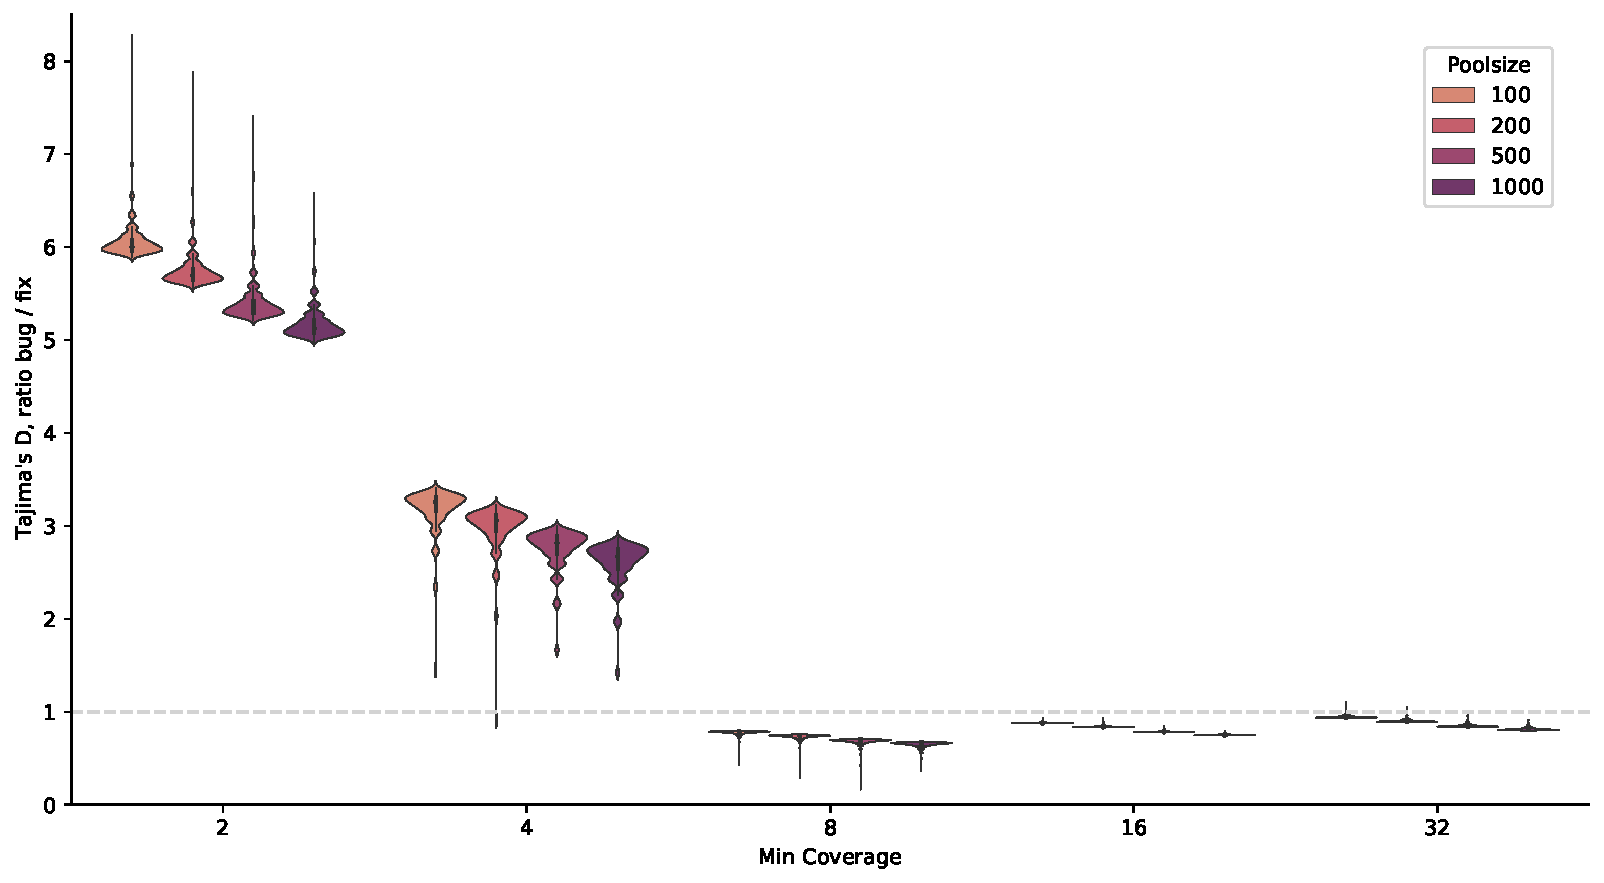
\includegraphics[width=\linewidth]{figures/bug-exam/window-100.pdf}
%     \vspace*{-1em}
%     \caption{
%         \textbf{Examination of the effect of the bugs in the computation of Tajima's D in PoPoolation.}
%         \\
%         Here, we show the overestimation of Tajima's D caused by the bugs in \toolname{PoPoolation} up to (and including) version v1.2.2. That is, we computed the the values for Tajima's D with and without the bug on randomly simulated test data, and here show the ratio of these two values to get the overestimation of the former compared to the latter. 
%         \\
%         The violin plots show the distributions of the overestimation across different windows (to capture stochasticity) with a window size of 100 base pairs. From left to right, we show groups of different minimum coverage values (the parameter \texttt{--min-coverage} set in \toolname{PoPoolation} for the computation, here: 2, 4, 8, 16, and 32). Within each group, we then show the effect of the pool size of the sample (here: %10, 20, 50, 
%         100, 200, 500, and 1000). %Note that \toolname{PoPoolation} (and \toolname{grenedalf}) have a limit for the minimum coverage based on the pool size; hence not all combinations are available here.
%         The dashed gray line is at a ratio of 1, which corresponds to the correct value where the computed values are identical.
%         In summary, each violin shows the overestimation of Tajima's for one combination of minimum coverage and pool size, where the violin shows the distribution of the overestimation across windows.
%         \\
%         We also ran this test with different window sizes (5, 10, 20, 50, 100, 200, 500, and 1000 base pairs). Overall, the overestimation is in the same range as shown here for all window sizes. For windows smaller than 100 base pairs, the overestimation tends to be somewhat higher, and with greater variance. For larger windows above 100 base pairs, the distributions get narrower, as the stochasticity within each window averages out. With windows of 200 base pairs and above, for the same min coverages and pool sizes shown here, the overestimation of Tajima's D converges to where the ``belly'' of each violin is in the plot.
%         \\
%         That means, when \toolname{PoPoolation} is run with its default value of 4 for the minimum coverage (option \texttt{--min-coverage}, the second group of violins), depending on pool size, the bug typically causes an overestimation of Tajima's D in the range of 2.8 to 3.5 times. For smaller minimum coverage, the effect is even worse.
%         % POOLSIZES="10 20 50 100 200 500 1000"
%         % MINCOVS="2 4 8 16 32"
%         % WINDOWS="5 10 20 50 100 200 500 1000"
%     }
% \label{fig:bug-exam}
% \end{figure*}

% In the implementation of the above $\tilde{D}_\text{pool}$,
% there are two bugs in \toolname{PoPoolation} $\leq$ v1.2.2, which alter the numerical results of the computation of Tajima's D.
% Firstly, they compute $\tilde{n}$ not by using the pool size $n$ and the coverage $C$ as stated above,
% but instead by using the pool size $n$ for both arguments, that is, mistakenly use $C := n$.
% Secondly, instead of computing $\alpha^*$ and $\beta^*$, they only compute $\beta^*$,
% and use this as the value for $\alpha^*$ as well.
% We have examined the effect of these bugs, and present results of the numerical changes induced by them
% in \todo{Supplementary document X}.

% \todo{maybe need to explain the two additional bugs here as well that i mentioned above}

%  \todo{@Lucas. Is it necessary to present plots of this? I think we can say this accounts of x percentage of error with coverage or number of individuals below x number}.


% ------------------------------------------------------------------------------------------------------
%          The Real Deal
% ------------------------------------------------------------------------------------------------------

\subsection{Conclusion and Comprehensive Approach}
\label{supp:sec:TajimaD:sub:RealDeal}

Above, the goal was to derive an estimator of Tajima's D for Pool-seq data which is quantitatively comparable to classical Tajima's D on individual data.  The overall difficulty is to find an estimator for the variance that we can use in \eqnref{eq:BasicTajimaD}.  
In a sense, there is a philosophical question about what Tajima's D even should be in the pool sequencing case, because the denominator should be the standard deviation (square root of the variance) of the numerator, but in the Pool-seq context, it is unclear what variance we mean.  Using the approach by Achaz, and plugging in the ``effective number of individuals sequenced'', as suggested by Kofler et al, is a somewhat reasonable idea, albeit not a perfect one. 

% Wow, I've had a hard time writing this in a way that does not make PoPoolation sound too bad... Jeff and I are still not sure whether the below is a bug in their code, a not well working aspect of their equations and statistics, or simply an oversight on their end... Hard to tell, and in dubio pro reo, I tried to write it as nicely as I could. I hope it works that way.

Firstly, the equations above leave it open what coverage to use for the computation of $\tilde{n}$ in \eqnref{eq:NTildeClosedForm} for computing the Achaz approach.  In \toolname{PoPoolation}, they use the minimum coverage $b$ as provided by the user, instead of empirical coverage in the window.  We suspect that this leads to a major distortion of the results:  As shown in \eqnref{eq:NTildeBounds}, the value of $\tilde{n}$ is bounded by both the coverage and the pool size; however, a requirement of the approach is that $b := 2$ (see \secref{supp:sec:TajimaD:sub:Classic}), which hence means that $\tilde{n} \leq 2$, which will rarely reflect the expected number of individuals sequenced.

Hence, empirical alternatives for the coverage likely yield more reasonable results. For instance, in order to use Tajima's D for outlier detection, one typically wants to be conservative. In that case, we should assume loci to be as correlated as possible, and hence use the smallest coverage in the given window instead, and plug that into the Achaz approach.

Furthermore, if we ignore all of the noise from pool sequencing, then the denominator should just be based on the equations by Achaz as explained above, but using the pool size $n$ instead of the effective pool size $\tilde{n}$.  This probably works well enough if coverage is high, as the noise induced by pool sequencing is relatively small compared to the noise introduced by demography (see below).  If however we want to include the noise from pool sequencing, which in particular is relevant at low coverages, then it becomes quite complicated, and the approach as described above starts to break down.

For a comprehensive estimator of the variance, we would have to know about the covariance of frequencies across sites. In the Pool-seq context, this has two components: (1) The first is a demographic component --- how has the randomness of the populations affected these two sites? The approach by Achaz answers that question (in isolation).  (2) The second is a Pool-seq component --- how does the randomness in the allele frequencies at these two sites covary?

These components are tricky to reconcile: By sequencing some subset of individuals at one site, and a different subset of individuals at another site, the estimated frequencies will covary in a different way than if the ``same'' subset of individuals were sequenced at both sites.  We would hence need to somehow integrate over the number of overlapping individuals for every pair of sites, which is not feasible with Pool-seq data.

Hence, finding a comprehensive solution that \emph{actually} yields the intended quantitatively comparable values of Tajima's D might involve knowledge of population history and simulations under a neutral model. We hence do not further pursue this approach at the time being.

In conclusion, we suggest the following: 

\begin{itemize}
    \item The approach of \toolname{PoPoolation} to use the minimum coverage $b$ to compute $\tilde{n}$ is likely not reasonable.
    \item Instead, using the pool size to replace the whole term, i.\,e., $\tilde{n} = n$, is better under high coverages.
    \item Alternatively, for a more conservative approach, we can compute $\tilde{n}$ as in \eqnref{eq:NTildeClosedForm}, by using pool size $n$, but set $c$ to the minimum empirical coverage found in the given window.
    \item By far the easiest and safest option in our opinion is to (for now) abandon the goal of quantitative comparability with the classic Tajima's D, and instead directly use the difference of $\theta_{\pi,\text{pool}}$ and $\theta_{w, \text{pool}}$.  As long as coverage is relatively equal along the regions being compared, this should enable the detection of outliers and other features of interest.
\end{itemize}

Lastly, we want to invite the research community to further scrutinize these approaches, and provide suggestions for how to move forward, in order to get a Pool-seq equivalent of Tajima's D that is quantitatively comparable to the classic estimator.

% ======================================================================================================
%          F_ST
% ======================================================================================================

\section{Fixation Index \texorpdfstring{\fst}{FST} for Pool-Seq}
\label{supp:sec:FST}

In this section, we will derive unbiased estimators of various measures of heterozygosity in two populations for Pool-sequencing data.
These will then be combined to obtain ``sample-size'' and ``pool-size'' corrected estimators of two definitions of \fst.
On top of these two estimators for \fst{} in the pool-sequencing context, we also walk through the two existing estimators as suggested by \citeay{Kofler2011b} and \citeay{Karlsson2007}.
Both are implemented in \toolname{PoPoolation2}, and are called the ``classical'' or ``conventional pool sequencing'' approach, and the ``Karlsson approach adapted to digital data'', respectively, in \citeay{Kofler2011b}.
We compare all four approaches to each other, and show that the ``classical'' approach is biased for lower coverages or small pool sizes, and the Karlsson approach is biased for small pool sizes (bias on the order of 1/pool size).
See also \citeay{Hivert2018} for an assessment of \fst{} in the pool-sequencing context.

% ------------------------------------------------------------------------------------------------------
%          Definition of F_ST
% ------------------------------------------------------------------------------------------------------

% \subsection{What the actual \texorpdfstring{F\textsubscript{(ST)}}{F(ST)}?}
\label{supp:sec:FST:sub:Definition}

There are several non-equivalent \emph{definitions} of $\text{F}_\text{ST}$.
The overall goal is to measure some degree of differentiation between two populations, which can be represented as a proportion of variation that cannot be explained by variation within populations.
What is unclear is a proportion of \emph{what} variation?
There are two natural candidates leading to two related, but distinct definitions of $\text{F}_\text{ST}$.
The first definition, which we will call $\text{F}_\text{ST}^\text{Nei}$ following \citeay{Nei1973}, considers the proportion of the total variation in the two populations.
This statistic is also called $\text{G}_\text{ST}$, see for example Equation (5.5) of \citeay{Hahn2018}.
The second definition, which we will call $\text{F}_\text{ST}^\text{Hudson}$ following \citeay{Hudson1992}, considers the proportion of the variation between populations, see also \citeay{Cockerham1969} and \citeay{Weir2002}.
This second definition is also considered in \citeay{Karlsson2007}, which we examine below in \secref{supp:sec:FST:sub:Karlsson}.

To make this more formal, we can consider the probability that two haploids carry different alleles.
We could consider drawing the two haploids from the same population (with the population chosen at random), which we call $\pi_\text{within}$; or we could consider drawing the two haploids from \emph{different} populations, which we call $\pi_\text{between}$; or finally we could consider drawing the two haploids totally at random from either population (potentially the same populations, potentially different populations) which we call $\pi_\text{total}$.
See \citeay{Bhatia2013} for more background information on this.

Our two definitions of $\text{F}_\text{ST}$ are then

\begin{align}
    \text{F}_\text{ST}^\text{Nei}    &:= 1 - \frac{\pi_\text{within}}{\pi_\text{total}} \label{eq:popnei}\\
    \text{F}_\text{ST}^\text{Hudson} &:= 1 - \frac{\pi_\text{within}}{\pi_\text{between}} \label{eq:pophudson}
\end{align}

If we consider a single locus with up $4$ alleles, with frequencies $f_{\tau(p)}$ (possibly zero) with  $\tau$ denoting the allele with $\tau \in \left\{A, C, G, T\right\}$ and $p$ denoting the population with subscripts $1$ and $2$, we can calculate the various $\pi$s as follows

\begin{align}
    \label{eq:PiDefs:PiWithin}
    \pi_\text{within} &= \frac{1}{2}\left[\left(1 - \sum_\tau f_{\tau(1)}^2\right) + \left(1 - \sum_\tau f_{\tau(2)}^2\right)\right] \\
    \label{eq:PiDefs:PiBetween}
    \pi_\text{between} &= 1 - \sum_\tau f_{\tau(1)}f_{\tau(2)} \\
    \label{eq:PiDefs:PiTotal}
    \pi_\text{total} &= \frac{1}{2}\pi_\text{within} + \frac{1}{2}\pi_\text{between}
\end{align}

which are then used in our above definitions of \fst.

% ------------------------------------------------------------------------------------------------------
%          Unbiased estimators of the Pi's
% ------------------------------------------------------------------------------------------------------

\subsection{Unbiased estimators of the \texorpdfstring{$\pi$s}{pi's}}
\label{supp:sec:FST:sub:EstimatorsPi}

Since both definitions of $\text{F}_\text{ST}$ rely on these $\pi$s, we will need to derive unbiased estimates for them.
We will show below that the following are unbiased estimators of the corresponding quantities without hats:

\begin{align}
    % \widehat{\pi}_\text{within} &=
    %     \frac{1}{2}
    %     \left[
    %           \left( \frac{n_{(1)}}{n_{(1)}-1} \right) \left( \frac{C_{(1)}}{C_{(1)}-1} \right) \left( 1 - \sum_{\tau} \left( \frac{c_{\tau(1)}}{C_{(1)}} \right)^2 \right)
    %         + \left( \frac{n_{(2)}}{n_{(2)}-1} \right) \left( \frac{C_{(2)}}{C_{(2)}-1} \right) \left( 1 - \sum_{\tau} \left( \frac{c_{\tau(2)}}{C_{(2)}} \right)^2 \right)
    %     \right] \\
    \nonumber
    % Some trickery is needed below for a nice alignment. Not quite perfect, but good enough for now.
    \widehat{\pi}_\text{within} &:=
        \frac{1}{2}
        \Bigg[                                 \left( \frac{n_{(1)}}{n_{(1)}-1} \right) \left( \frac{\coverage_{(1)}}{\coverage_{(1)}-1} \right) \left( 1 - \sum_{\tau} \empfreq_{\tau(1)}^2 \right) \Bigg. \\
    \label{eq:Fst:UnbiasedPiWithin}
        \Bigg. &+ \phantom{\frac{1}{2} \Bigg[} \left( \frac{n_{(2)}}{n_{(2)}-1} \right) \left( \frac{\coverage_{(2)}}{\coverage_{(2)}-1} \right) \left( 1 - \sum_{\tau} \empfreq_{\tau(2)}^2 \right) \Bigg] \\
    \label{eq:Fst:UnbiasedPiBetween}
    \widehat{\pi}_\text{between} &:=
        1 - \sum_{\tau} \empfreq_{\tau(1)}\empfreq_{\tau(2)} \\
    \label{eq:Fst:UnbiasedPiTotal}
    \widehat{\pi}_\text{total} &:=
        \frac{1}{2}\widehat{\pi}_\text{within} + \frac{1}{2}\widehat{\pi}_\text{between}
\end{align}

In the following, we derive these estimators.

% --------------------------------------------------------
%          Pi Within
% --------------------------------------------------------

\subsubsection*{Unbiased estimator of \texorpdfstring{$\widehat{\pi}_\text{within}$}{Pi Within}}
\label{supp:sec:FST:sub:EstimatorsPi:sub:PiWithin}

We have derived previously that
\[
\mathbb{E}\left[\left(\frac{n_{(1)}}{n_{(1)}-1}\right)\left(\frac{\coverage_{(1)}}{\coverage_{(1)}-1}\right)\left(1 - \sum_{\tau}\empfreq_{\tau(1)}^2\right) \right] = \left(1 - \sum_\tau f_{\tau(1)}^2\right)
\]
within a single population.  It follows immediately that averaging these estimators across the two populations is unbiased for $\pi_\text{within}$.

% --------------------------------------------------------
%          Pi Between
% --------------------------------------------------------

\subsubsection*{Unbiased estimator of \texorpdfstring{$\widehat{\pi}_\text{between}$}{Pi Between}}
\label{supp:sec:FST:sub:EstimatorsPi:sub:PiBetween}

Since the two pools are independent, we have that
\[
\mathbb{E}\left[\widehat{\pi}_\text{between}\right] = 1- \sum_\tau \mathbb{E}\left[\empfreq_{\tau(1)}\right]\mathbb{E}\left[\empfreq_{\tau(2)}\right]
\]
The frequency of alleles within a pool is an unbiased estimate for the frequency in the population, so
\[
\mathbb{E}\left[\empfreq_{\tau(p)}\right] = f_{\tau(p)}
\]
showing that $\widehat{\pi}_\text{between}$ is unbiased for $\pi_\text{between}$.

% --------------------------------------------------------
%          Pi Total
% --------------------------------------------------------

\subsubsection*{Unbiased estimator of \texorpdfstring{$\widehat{\pi}_\text{total}$}{Pi Total}}
\label{supp:sec:FST:sub:EstimatorsPi:sub:PiTotal}

That $\widehat{\pi}_\text{total}$ is unbiased for $\pi_\text{total}$ follows immediately from the definition of $\pi_\text{total}$ in \eqnref{eq:PiDefs:PiTotal} and the unbiasedness of $\widehat{\pi}_\text{within}$ and $\widehat{\pi}_\text{between}$.

% --------------------------------------------------------
%          Intuition about the equations
% --------------------------------------------------------

\subsubsection*{Intuition and Reasoning}
\label{supp:sec:FST:sub:EstimatorsPi:sub:Intuition}

In the above equations, for each of the two populations, we apply a double Bessel's correction for our estimate of $\widehat{\pi}_\text{within}$ in \eqnref{eq:Fst:UnbiasedPiWithin}, to correct for the elevated variance that comes from the double sampling process of picking individuals from a population, and of picking reads from those individuals (during sequencing). Because in both steps, we pick finite numbers, resulting in higher variance in the estimates, which hence needs correcting. 

However, the estimate of $\widehat{\pi}_\text{between}$ in \eqnref{eq:Fst:UnbiasedPiBetween} does not have those corrections. One way to gain some intuition about why the Bessle's corrections are not needed in that case is as follows.

One way to think about $\pi$ in a single population is as the probability to get different alleles when picking two random haploids from the population.  In a large population, it does not matter whether we pick those two haploids with replacement or without replacement: in that case, even if we pick the two haploids with replacement, it is unlikely that we would happen to pick the same haploid twice.  In that sense, $\pi$ is measuring the probability that two different haploids have different alleles.  
 
Now, to estimate the population-level $\pi_\text{within}$, we could look at a smaller sample of haploids, and calculate the probability that two randomly chosen haploids have different alleles. However, if our sample size is small, then the difference between sampling with or without replacement becomes relevant, because there is a $\sfrac{1}{n}$ chance that we pick the same haploid twice if we are sampling with replacement. If we pick the same haploid twice, they obviously cannot have different alleles.  This means that if we compute our probabilities by sampling with replacement, then we underestimate by a factor of $1 - \sfrac{1}{n} = \frac{n-1}{n}$ because in $\sfrac{1}{n}$ of our comparisons we are actually comparing a haplotype to itself.  As a result, we would need to multiply our estimate by $\frac{n}{n-1}$ to undo this underestimation.  Something similar happens again when we move to pool sequencing, where our equations are (implicitly) in terms of sampling with replacement, but now we are sampling reads, and so we end up (by the same argument) with needing to multiply by a factor of $\frac{c}{c-1}$.  

This however is different in the case of $\pi_\text{between}$.  In that case, we are comparing a haploid from one population to a haploid from a different population.  Hence, we are comparing a single haploid (or single read) from one population to a single haploid (or read) from another population.  If we only draw a single sample, then there is no difference between sampling with or without replacement, and so our equations (which again are implicitly based on sampling with replacement) do not need to be corrected to match the idea of sampling without replacement.  

In summary, when considering two entities at a time from the same pool/population, we need to include Bessel's corrections such as for pool size and read coverage. However, if we are only considering one entity at a time from each pool/population, then we do not need those corrections.

% ------------------------------------------------------------------------------------------------------
%          Estimating FST
% ------------------------------------------------------------------------------------------------------

\subsection{Final asymptotically unbiased estimators of \texorpdfstring{$\text{F}_\text{ST}$}{FST} per SNP and per window}
\label{supp:sec:FST:sub:EstimatorFST}

These estimators then immediately suggest the following ratio estimators for the different definitions of $\text{F}_\text{ST}$:

\begin{align}
    \widehat{\text{F}}_\text{ST}^\text{Nei} &:= 1 - \frac{\widehat{\pi}_\text{within}}{\widehat{\pi}_\text{total}}\\
    \widehat{\text{F}}_\text{ST}^\text{Hudson} &:= 1 - \frac{\widehat{\pi}_\text{within}}{\widehat{\pi}_\text{between}}
\end{align}

All of this has been for a single site, but we are often interested in combining information across SNPs within a window $W$ (or possibly genome wide).
In such a case, define $\widehat{\pi}^\ell_\text{within}$ to be $\widehat{\pi}_\text{within}$ as above but for SNP $\ell \in W$.
Define $\widehat{\pi}^\ell_\text{between}$ and $\widehat{\pi}^\ell_\text{total}$ analogously.
We then combine information across the SNPs in the window $W$ as

\begin{align}
    \widehat{\text{F}}_\text{ST}^\text{Nei}    &= 1 - \frac{\sum_{\ell \in W} \widehat{\pi}^\ell_\text{within}} {\sum_{\ell \in W} \widehat{\pi}^\ell_\text{total}} \\
    \widehat{\text{F}}_\text{ST}^\text{Hudson} &= 1 - \frac{\sum_{\ell \in W} \widehat{\pi}^\ell_\text{within}} {\sum_{\ell \in W} \widehat{\pi}^\ell_\text{between}}
\end{align}

See \citeay{Bhatia2013} for a practical and theoretical justification for using this ``ratio of averages'' instead of using an ``average of ratios''.
These are our asymptotically unbiased estimators for \fst{} for Pool-seq data, which take the finite sampling of individuals from the population, and the finite sampling of reads from each individual in the pool, into account.

% ------------------------------------------------------------------------------------------------------
%          PoPoolation2 Estimator of FST
% ------------------------------------------------------------------------------------------------------

\subsection{Estimator of \texorpdfstring{$\text{F}_\text{ST}$}{FST} as implemented in PoPoolation2}
\label{supp:sec:FST:sub:PoPoolation2Estimator}

The implementation in \toolname{PoPoolation2} \cite{Kofler2011b} offers two ways to estimate \fst{}:
What they call the ``classical'' or ``conventional'' approach by \citeay{Hartl2007}, and an approach adapted to digital data following \citeay{Karlsson2007}.
In this and the next section, we discuss these estimators.
We later show that they are biased, and hence recommend using the estimates as introduced above instead.
For comparability and historical backwards compatibility, we however still offer both these estimators in our implementation in \toolname{grenedalf}.

% \todo{see if we actually get to do this in time:}
% Furthermore, the PoPoolation equations document explains derivations of equations for Pool-seq corrected estimators of \fst, which however to the best of our knowledge are not actually implemented in either \toolname{PoPoolation} nor \toolname{PoPoolation2}.
% We here still walk through these, see \secref{supp:sec:PoPoolation2Equations}.

First, we present the ``classical'' approach as implemented in \toolname{PoPoolation2}, labelled with superscript ``Kofler'' here, following \citeay{Kofler2011b}.
We compute \fst{} for two subpopulations, which we here again denote with subscripts $(1)$ and $(2)$, and the total population with $(T)$. We expect poolsizes $n >= 2$.

For each SNP in a given window, \toolname{PoPoolation2} computes:
% \verb|f_st_conventional_pool_pi_snp|

\begin{align}
    \label{eq:PoPoolation2FstPi:1}
    \widehat{\pi}_{(1)}^\text{Kofler}  &:= \frac{\coverage_{(1)}}{\coverage_{(1)}-1} \cdot  \left( 1 - \sum_\tau \empfreq_{\tau(1)}^2 \right) \\
    \label{eq:PoPoolation2FstPi:2}
    \widehat{\pi}_{(2)}^\text{Kofler}  &:= \frac{\coverage_{(2)}}{\coverage_{(2)}-1} \cdot  \left( 1 - \sum_\tau \empfreq_{\tau(2)}^2 \right) \\
    \label{eq:PoPoolation2FstPi:T}
    \widehat{\pi}_{(T)}^\text{Kofler}  &:= \frac{\coverage_{(T)}}{\coverage_{(T)}-1} \cdot  \left( 1 - \sum_\tau \empfreq_{\tau(T)}^2 \right) \\
    \nonumber
    \mbox{with} \\
    \nonumber
    \coverage_{(T)} &:= \mbox{min} \left( \coverage_{(1)}, \coverage_{(2)} \right) \\
    \nonumber
    \empfreq_{\tau(T)} &:= \frac{1}{2} \left( \empfreq_{\tau(1)} + \empfreq_{\tau(2)} \right)
\end{align}

These quantities are accumulated over the window $W$, with $(\ell)$ denoting the above at SNP $\ell$
% \verb|f_st_conventional_pool|

\begin{align}
    \label{eq:PoPoolation2FstWindow:1}
    \widehat{\pi}_{W(1)}^\text{Kofler} &= \frac{n_{(1)}}{n_{(1)}-1} \cdot \sum_{\ell\in W} \widehat{\pi}_{(1)}^\text{Kofler}(\ell)\\
    \label{eq:PoPoolation2FstWindow:2}
    \widehat{\pi}_{W(2)}^\text{Kofler} &= \frac{n_{(2)}}{n_{(2)}-1} \cdot \sum_{\ell\in W} \widehat{\pi}_{(2)}^\text{Kofler}(\ell)\\
    \label{eq:PoPoolation2FstWindow:T}
    \widehat{\pi}_{W(T)}^\text{Kofler} &= \frac{n_{(T)}}{n_{(T)}-1} \cdot \sum_{\ell\in W}  \widehat{\pi}_{(T)}^\text{Kofler}(\ell)\\
    \nonumber
    \mbox{with} \\
    \nonumber
    n_{(T)} &= \mbox{min} \left( n_{(1)}, n_{(2)} \right)
\end{align}

Finally, the estimate of \fst is computed as:

\begin{align}
    \label{eq:PoPoolation2FstEst}
    \widehat{\text{F}}_\text{ST}^\text{Kofler} &= \frac{ \widehat{\pi}_{W(T)}^\text{Kofler} - \frac{1}{2} \left(     \widehat{\pi}_{W(1)}^\text{Kofler} +     \widehat{\pi}_{W(2)}^\text{Kofler}  \right)}{ \widehat{\pi}_{W(T)}^\text{Kofler}}
\end{align}

Note that following the notation of the previous section, $\frac{1}{2}\left(\widehat{\pi}_{W(1)}^\text{Kofler} + \widehat{\pi}_{W(2)}^\text{Kofler}\right)$ is identical to the windowed version of $\widehat{\pi}_\text{within}$ and hence is unbiased.  Unfortunately, $\widehat{\pi}_{W(T)}^\text{Kofler}$ however is not an unbiased estimator of $\pi_\text{total}$.  There are two main issues.  First, recall that $\pi_\text{total} = \frac{1}{2}\left(\pi_\text{between}  + \pi_\text{within} \right)$.  The naive estimator of $\pi_\text{between}$ turns out to be unbiased as shown in the previous section, but yet in the PoPoolation estimator, there is a Bessel correction acting on the whole estimator --- this effectively biases the contribution of the part estimating $\pi_\text{between}$ upward.  Second, $\pi_\text{within}$ has two components corresponding to the two populations.  Since these have different coverages and different sample sizes, the components estimating each of these have different biases that need to be corrected separately.  Instead, PoPoolation uses the minimum coverage and the minimum sample size for both.  This again will result in an upward bias for the sample with higher coverage and/or larger pool size.  Overall, these two errors can result in substantial upward bias for $\widehat{\pi}_{W(T)}^\text{Kofler}$, which will result in substantial upward bias for $\widehat{\text{F}}_\text{ST}^\text{Kofler}$, as we show later.  This was also pointed out by \citeay{Hivert2018}. It is therefore recommended to use the estimator presented in the previous section instead.

% Moi's rendering of the equations. Keeping it here for reference, in case it's later needed.

% We create an unbiased estimator based on $\text{F}_\text{ST}$'s definition based on nucleotide diversity within a sub-population $S$ and across a total set of populations $T$ (see Equation (5.5) of \citeay{Hahn2018}):
% \begin{align}
%     \text{F}_\text{ST} &= \frac{\theta_{\pi,T} - \theta_{\pi,S}}{\theta_{\pi,T}}
% \end{align}
% Since we have already derived unbiased estimators for $\theta_\pi$, given two libraries of DNA sequences from two Pool-seq populations with their corresponding $u$ alternative alleles, $v$ reference alleles, $C$ coverages, and $n$ individuals, we can calculate:
% \begin{align}
%   \text{F}_\text{ST} &=
%     \frac{
%         \theta_\pi(u_1+u_2,v_1+v_2,C_1+C_2,n_1+n_2) -
%         \frac{1}{2}(
%             \theta_\pi(u_1,v_1,C_1,n_1) +
%             \theta_\pi(u_2,v_2,C_2,n_2)
%         )
%     }{
%      \theta_\pi(u_1+u_2,v_1+v_2,C_1+C_2,n_1+n_2)
%     }
% \end{align}

% ------------------------------------------------------------------------------------------------------
%          FST Asymptotically Unbiased, Karlsson
% ------------------------------------------------------------------------------------------------------

\subsection{Asymptotically Unbiased Estimator of \texorpdfstring{\fst}{FST} by Karlsson \textit{et al.}}
\label{supp:sec:FST:sub:Karlsson}

Another estimator for \fst{} that is offered in \toolname{PoPoolation2} is based on the equations used in \citeay{Karlsson2007}, see the last page of the Supplemental Information of Karlsson \textit{et al.} for their derivation.
We here briefly also go through the derivation.
% We also offer this estimator in our implementation, and briefly derive it here.

We here call this estimator using the superscript ``Karlsson'', which is again defined for two subpopulations denoted with subscripts $(1)$ and $(2)$.
% We expect poolsizes $n >= 2$.
We are here only looking at biallelic SNPs.
Instead of $\tau$ for the four nucleotides, we hence use $q$ for the frequency of the major (reference) allele and $p$ for the frequency of the minor (alternative) allele.  We will also use $\widehat{q}$ and $\widehat{p}$ as the corresponding empirical estimates of $q$ and $p$ (\ie the number of reads supporting the major or minor allele divided by the coverage).

We start with the definition of $\text{F}_\text{ST}^\text{Karlsson}$ from Karlsson \textit{et al.} for the SNPs in a window $W$:

\begin{align}
    \label{eq:FstK}
    \text{F}_\text{ST}^\text{Karlsson} &= \frac{\sum_W N_k}{\sum_W D_k}
\end{align}

where the the numerator $N_k$ and denominator $D_k$ for a single site $k$ in $W$ are:

\begin{align}
    \label{eq:FstNk}
    N_k &= p_{(1)} \cdot ( q_{(2)} - q_{(1)} ) ~+~ p_{(2)} \cdot ( q_{(1)} - q_{(2)} ) \\
    \label{eq:FstDk}
    \nonumber
    D_k &= p_{(1)} q_{(2)} + q_{(1)} p_{(2)} \\
        &= N_k + p_{(1)} q_{(1)} + p_{(2)} q_{(2)}.
\end{align}

It is not obvious, but follows from simple algebra that this definition is equivalent to $ \text{F}_\text{ST}^\text{Hudson} $ defined above.

These are estimated as follows, using the numerator $\hat{N}_k$ and denominator $\hat{D}_k$ at a single site:

\begin{align}
    \label{eq:FstKnh}
    \widehat{N}_k &= \left( \widehat{q}_{(1)} - \widehat{q}_{(2)} \right)^2 - \left( \frac{h_{(1)}}{\coverage_{(1)}} + \frac{h_{(2)}}{\coverage_{(2)}} \right) \\
    \label{eq:FstKdh}
    \widehat{D}_k &= \widehat{N}_k + h_{(1)} + h_{(2)}
    \intertext{with two additional helpers:}
    \nonumber
    h_{(1)} &= \frac{\coverage_{(1)}}{(\coverage_{(1)}-1)}\widehat{q}_{(1)}\widehat{p}_{(1)} \\
    \nonumber
    h_{(2)} &= \frac{\coverage_{(2)}}{(\coverage_{(2)}-1)}\widehat{q}_{(2)} \widehat{p}_{(2)}
    \end{align}

And finally, these are used to define estimator $\widehat{\text{F}}_\text{ST}^\text{Karlsson}$ for a window $W$:

\begin{align}
    \label{eq:FstEstK}
    \widehat{\text{F}}_\text{ST}^\text{Karlsson} &= \frac{\sum_W \widehat{N}_k}{\sum_W \widehat{D}_k}
\end{align}

According to Karlsson \textit{et al.}, when the coverages $\coverage_{(1)}$ and $\coverage_{(2)}$ (called ``sample sizes'' there) are equal, the estimator reduces to the estimator of \fst{} given by \citeay{Weir2002}.
Karlsson \textit{et al.} further state that by the Lehmann-Scheff\'{e} theorem \cite[Theorem 4.2.2]{Bickel1977}, it follows that $\widehat{N}_k$ and $\widehat{D}_k$ are uniformly minimum variance unbiased estimators of $N_k$ and $D_k$, respectively, and hence conclude that their estimator \^{F}\textsubscript{ST,K} is also asymptotically unbiased.

This estimator is very similar (after some algebra) to our $\widehat{\text{F}}_\text{ST}^\text{Hudson}$.
It however assumes the pool size to be infinite, that is, it is missing the corrections for pool size.

% ------------------------------------------------------------------------------------------------------
%          Comparison of the Estimators and their Biases
% ------------------------------------------------------------------------------------------------------

\subsection{Comparison of the Estimators and their Biases}
\label{supp:sec:FST:sub:Comparison}

As mentioned above, both the Kofler estimator in \toolname{PoPoolation2} and the Karlsson estimator have biases.
We here explore their effects via simulations, and further show that our estimators are approximately unbiased under the Pool-seq assumptions so long as sequencing error rates are low.

% --------------------------------------
%     Simulation Setup
% --------------------------------------

\subsubsection*{Simulation Setup}
\label{supp:sec:FST:sub:Comparison:sub:Simulations}

To test the accuracy of the different estimators of $\text{F}_\text{ST}$ we performed two sets of simulations.  In both sets of simulations we assumed a biallelic mutation model, and a simple model of sequencing.  Our sequencing model assumes that (1)~each position is independent, (2)~the number of reads at a given position is Poisson distributed with the mean of that distribution being the ``Read Depth'' of that simulation, (3)~each read is equally likely to come from any individual in the pool, and (4)~with probability ``Seq Error'' a read shows the opposite allele as the individual it was sampled from, but otherwise matches the individual's allele, and this error process is independent across reads.  Across both sets of simulations, we vary the sequencing error in $\left\{0, 10^{-5}, 10^{-4}, 10^{-3}\right\}$, the number of haploid individuals in the pool in $\left\{10, 100, 1000\right\}$, and the mean sequencing depth in $\left\{10, 100, 1000\right\}$.  In both sets of simulations, we obtain population-level allele frequencies at each site, and then compute the true values of either $\neifst$ or $\hudsonfst$ using \cref{eq:popnei,eq:pophudson,eq:PiDefs:PiWithin,eq:PiDefs:PiTotal,eq:PiDefs:PiBetween}.
We here use ``0'' and ``1'' to denote the major and minor allele, respectively.

In the first set of simulations, which we call the ``simple'' simulations, we simulate 1000 sites in two populations.  Let $f_j^{(p)}$ be the frequency of one of the ``1'' allele at position $j$ in population $p$.  To obtain correlated allele frequencies in the two populations we simulated the frequencies as
\begin{align*}
f_j^{(1)} &\overset{i.i.d.}{\sim} \text{Beta}(0.1, 0.5) \\
f_j^{(2)} | f_j^{(1)} &\sim \text{Beta}\left(\frac{\gamma f^{(1)}_j}{1-f^{(1)}_j+10^{-10}}, \gamma\right),
\end{align*}
where $\gamma$ controls the degree of correlation between the frequencies in the two populations.  As $\gamma$ increases, the correlation between the frequencies decreases.  This parameterization is chosen so that $\mathbb{E}\left[f_j^{(2)} \mid f_j^{(1)}\right] = f_j^{(1)}$ up to the error introduced by the $10^{-10}$ which is included for numerical stability.  Then, to obtain the frequency of the ``1'' allele in our pool, we performed independent binomial sampling at each site for each population.  Finally, we obtained the number of reads with the ``0'' and ``1'' alleles as described above.  We varied $\gamma$ in $\left\{0.1, 0.325, 0.55, 0.775, 1\right\}$, and performed 10 simulations each for each setting of $\gamma$, sequencing error, pool size, and sequencing depth, resulting in 1800 simulations.

In the second set of simulations we used \texttt{msprime} \citep{baumdicker2022efficient,kelleher2016efficient} to simulate data under a population genetic model.  In this model, we simulate two populations of constant size that diverged at a time, $t_\text{div}$, in the past, with the ancestral population having the same, constant size.  Across simulations, we varied $t_\text{div}$ in $\left\{0, 0.25, 0.5, 0.75, 1.0\right\}$.  We used a population-scaled mutation rate, $\theta$, of $0.001$, a population-scaled recombination rate, $\rho$, of $0.0001$, and simulated sequences of length $1$ Mb.  Since \texttt{msprime} is a coalescent simulator, it samples individual-level data.  As such, for a given simulation we directly obtain the alleles of the individuals at each of the $10^6$ sites for the individuals that make up our pool sequencing sample.  We then draw reads for each of those sites as described above.  To obtain population-level allele frequencies we simulate an additional 1000 haploid individuals in each population beyond those that make up the pool, and we use the empirical frequencies of the alleles in this 1000 $+$ pool size sample as the ``true'' allele frequencies in each population.

% --------------------------------------
%     valuation and Results
% --------------------------------------

\subsubsection*{Evaluation and Results}
\label{supp:sec:FST:sub:Comparison:sub:Results}

\begin{figure*}[p]
    \centering
    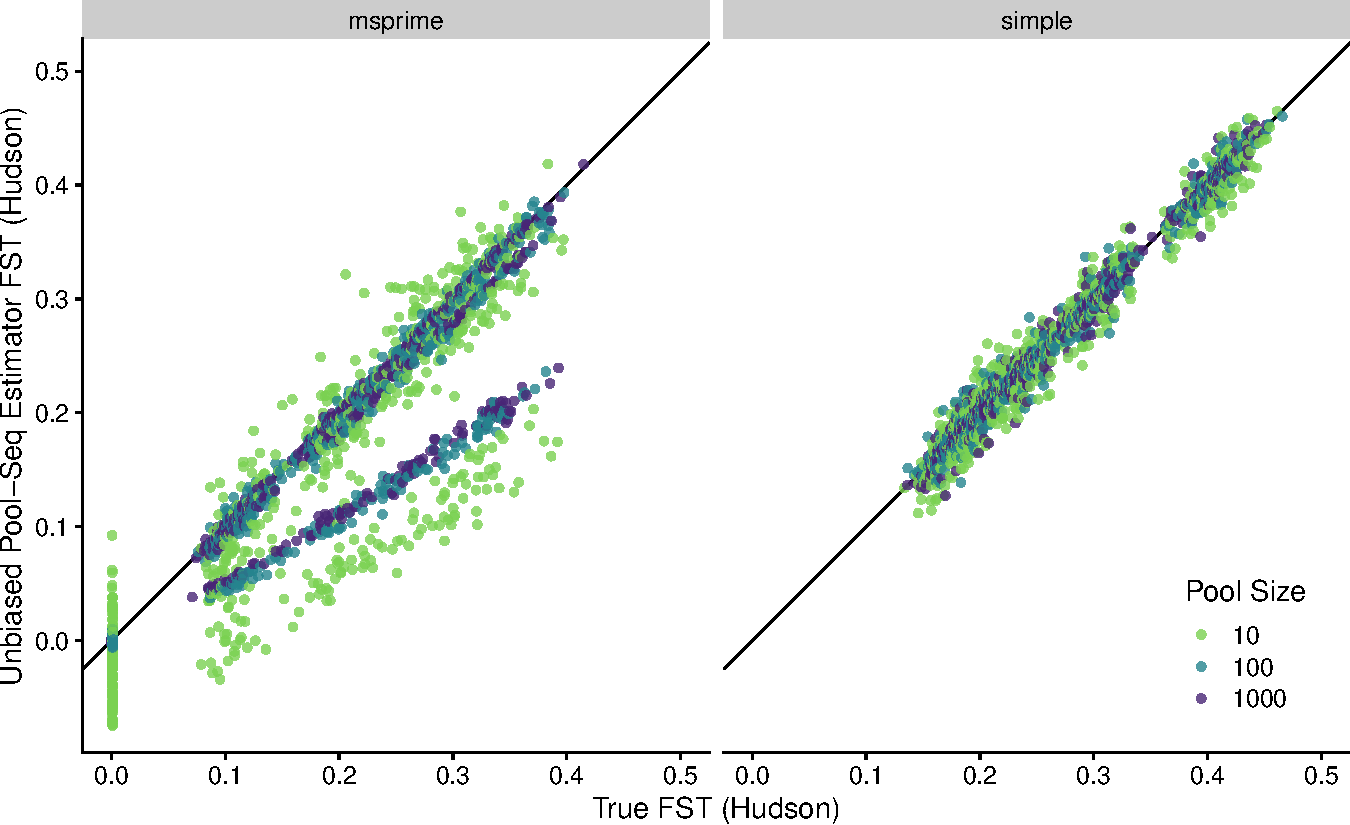
\includegraphics[width=.69\linewidth]{true_hudson_fst-est_spence_hudson-pool_size.pdf}
    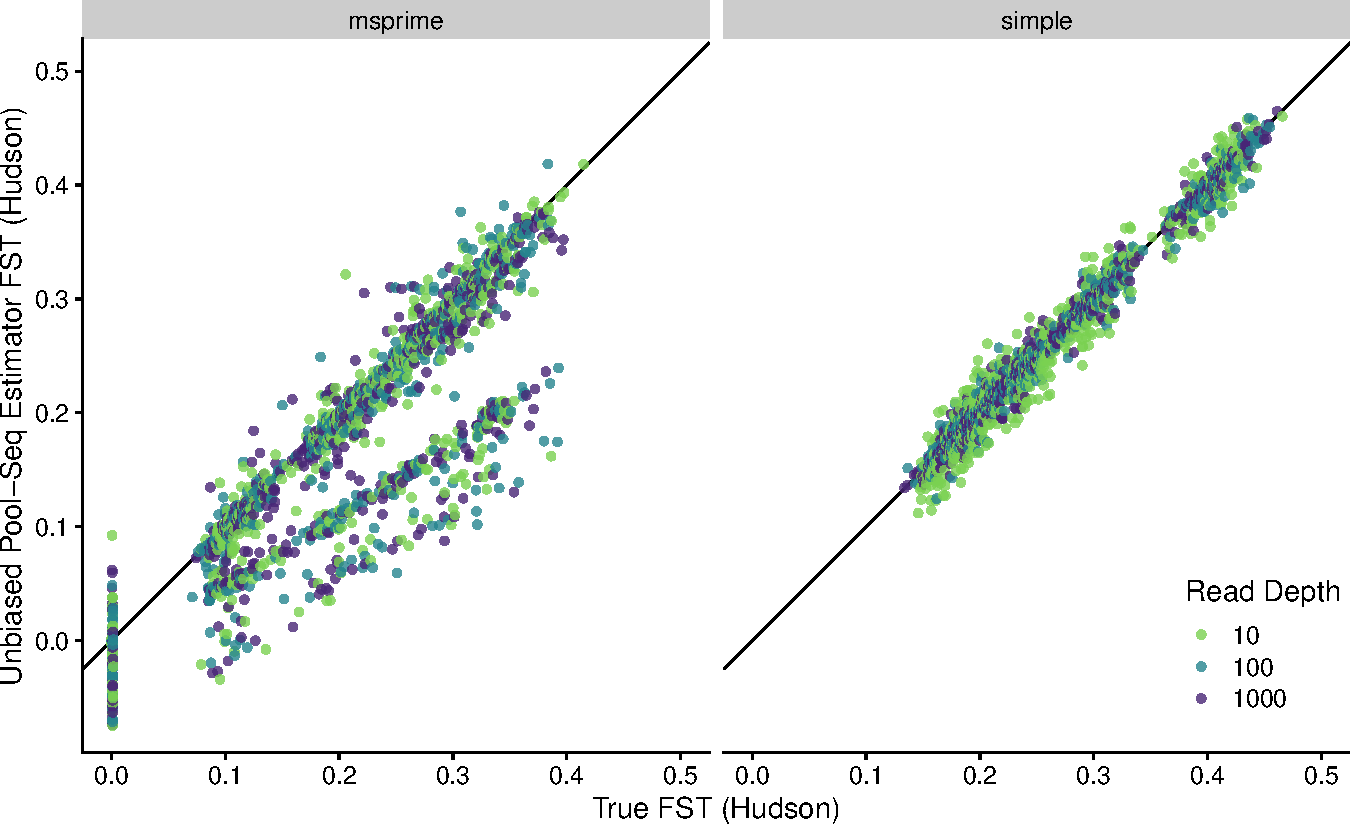
\includegraphics[width=.69\linewidth]{true_hudson_fst-est_spence_hudson-read_depth.pdf}
    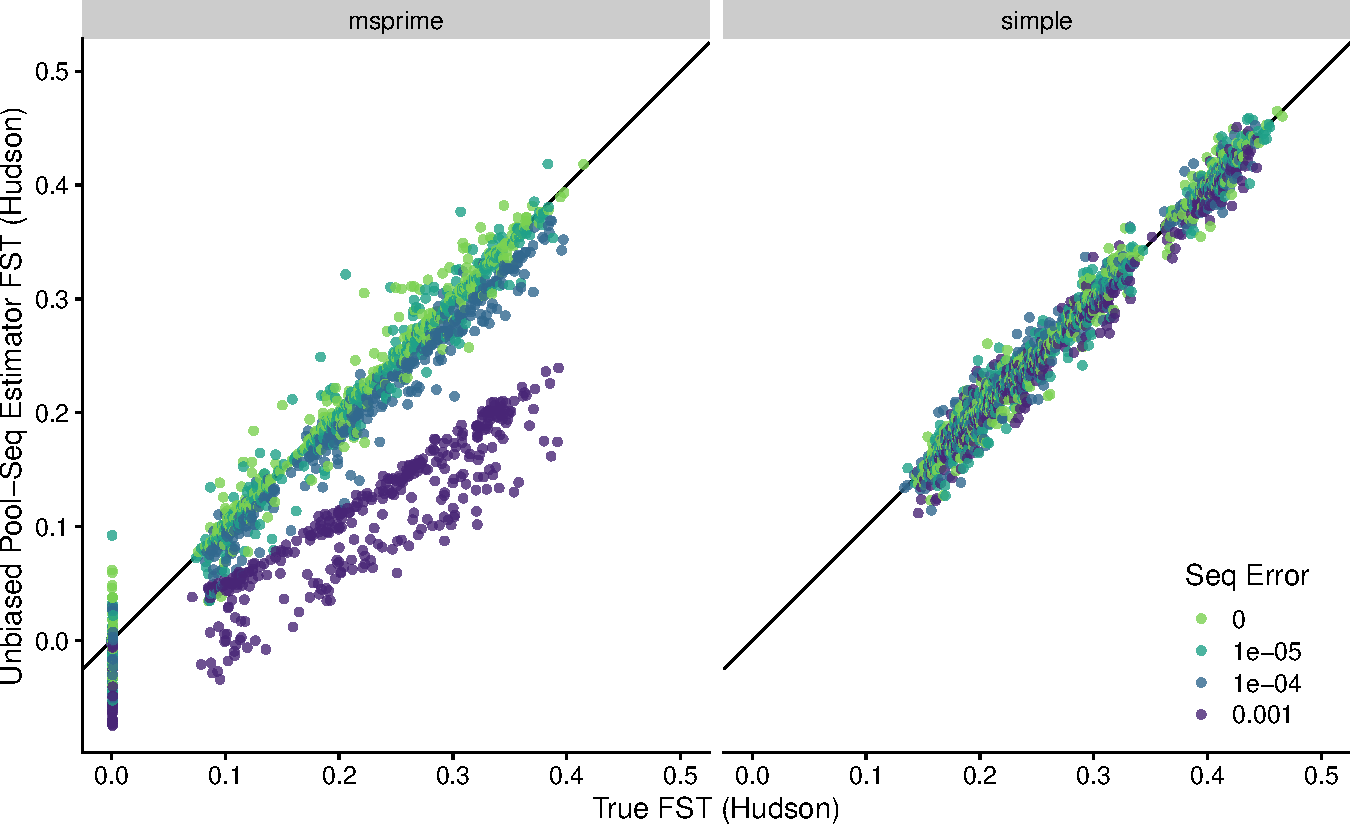
\includegraphics[width=.69\linewidth]{true_hudson_fst-est_spence_hudson-seq_error.pdf}
    \vspace*{-1em}
    \caption{
%         \textbf{Unbiased Hudson}
        Unbiased Pool-Seq Estimator for FST (Hudson) vs true FST (Hudson).
    }
\label{fig:UnbiasedHudson}
\end{figure*}

\begin{figure*}[p]
    \centering
    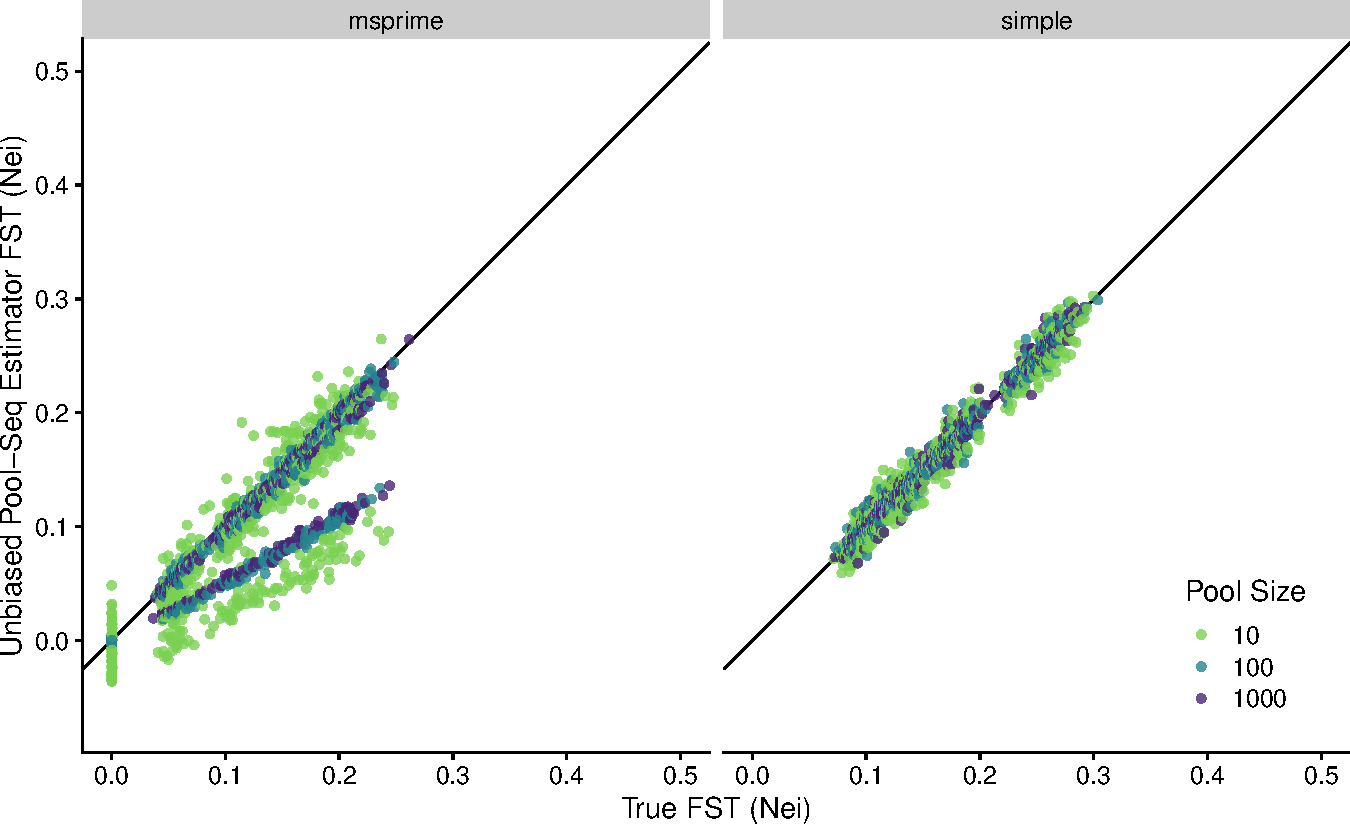
\includegraphics[width=.69\linewidth]{true_nei_fst-est_spence_nei-pool_size.pdf}
    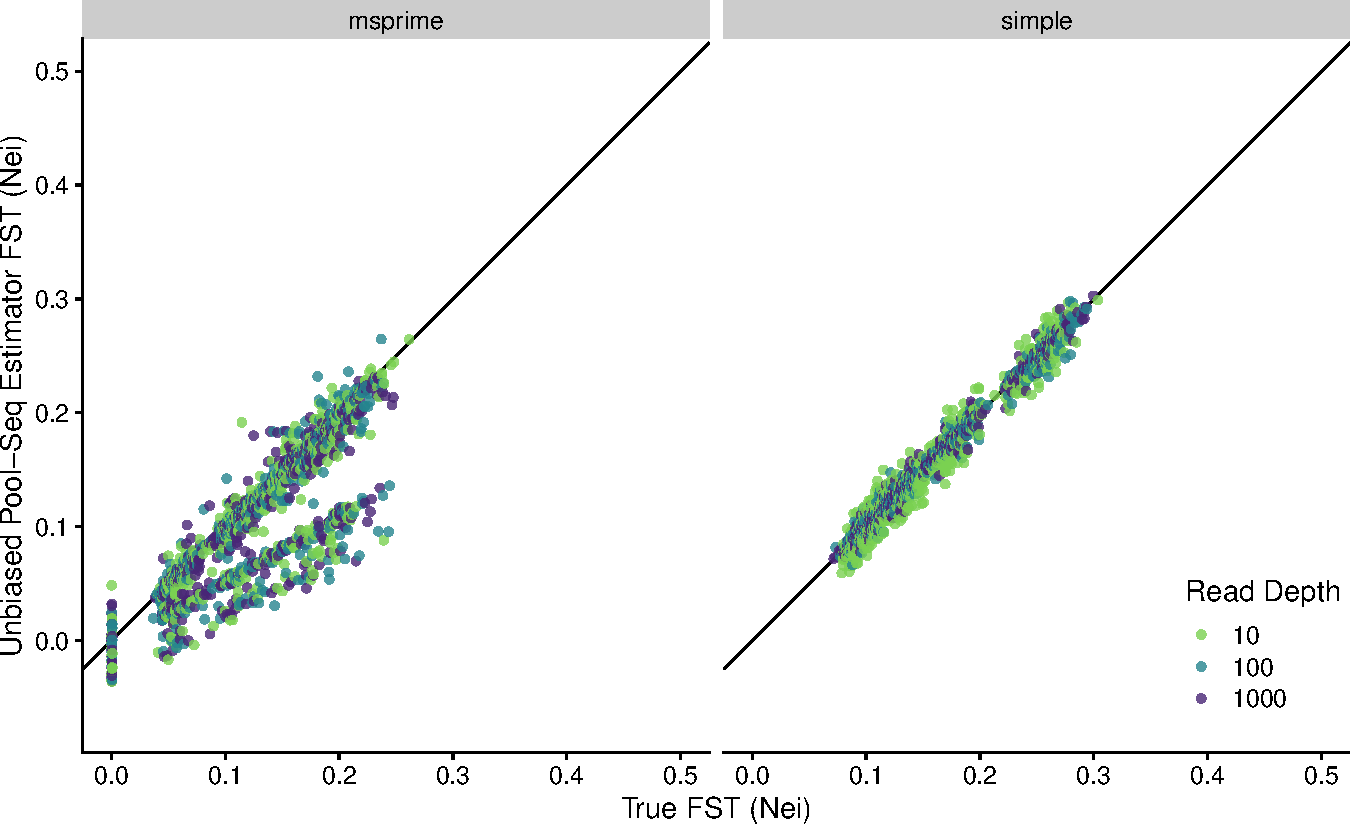
\includegraphics[width=.69\linewidth]{true_nei_fst-est_spence_nei-read_depth.pdf}
    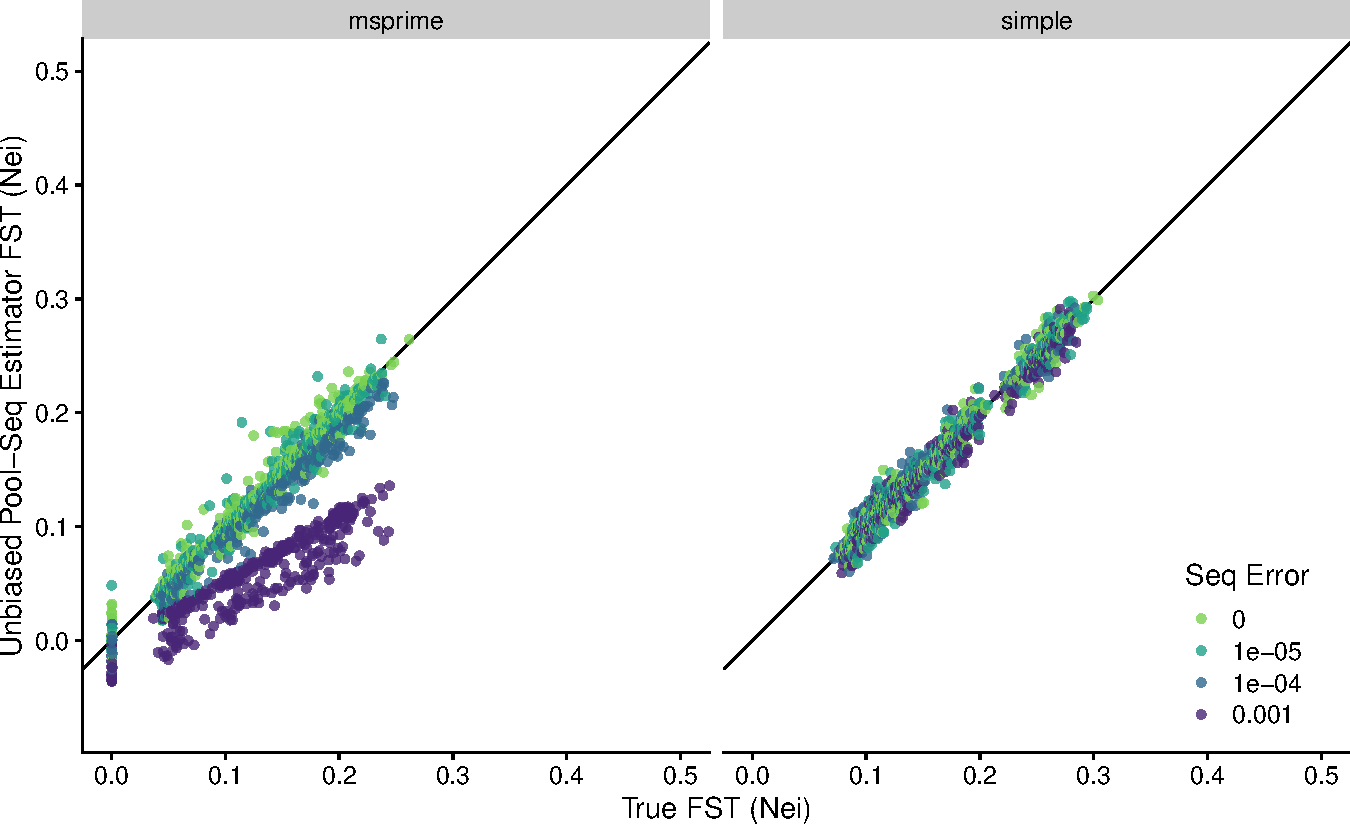
\includegraphics[width=.69\linewidth]{true_nei_fst-est_spence_nei-seq_error.pdf}
    \vspace*{-1em}
    \caption{
%         \textbf{Unbiased Nei}
        Unbiased Pool-Seq Estimator for FST (Nei) vs true FST (Nei).
    }
\label{fig:UnbiasedNei}
\end{figure*}

\begin{figure*}[p]
    \centering
    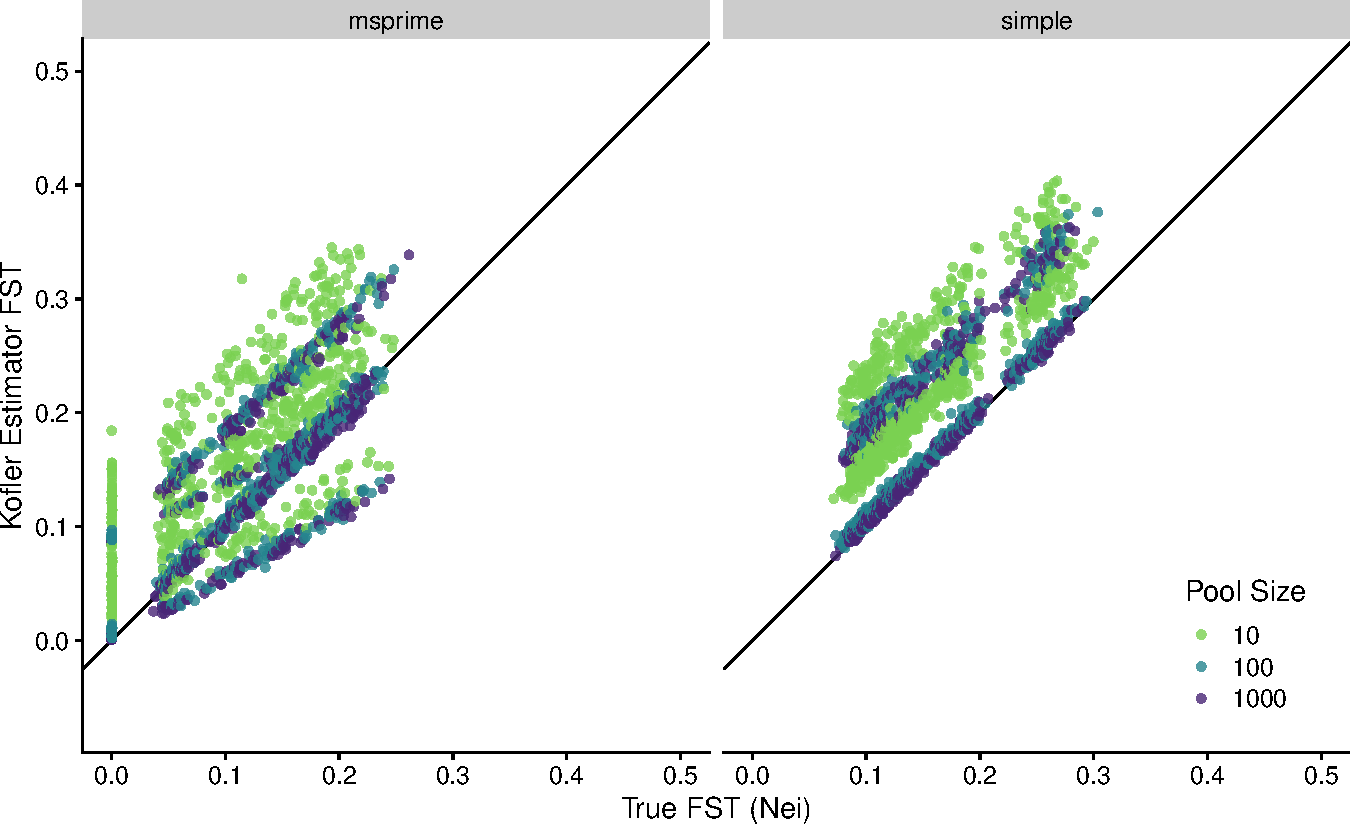
\includegraphics[width=.69\linewidth]{true_nei_fst-est_kofler-pool_size.pdf}
    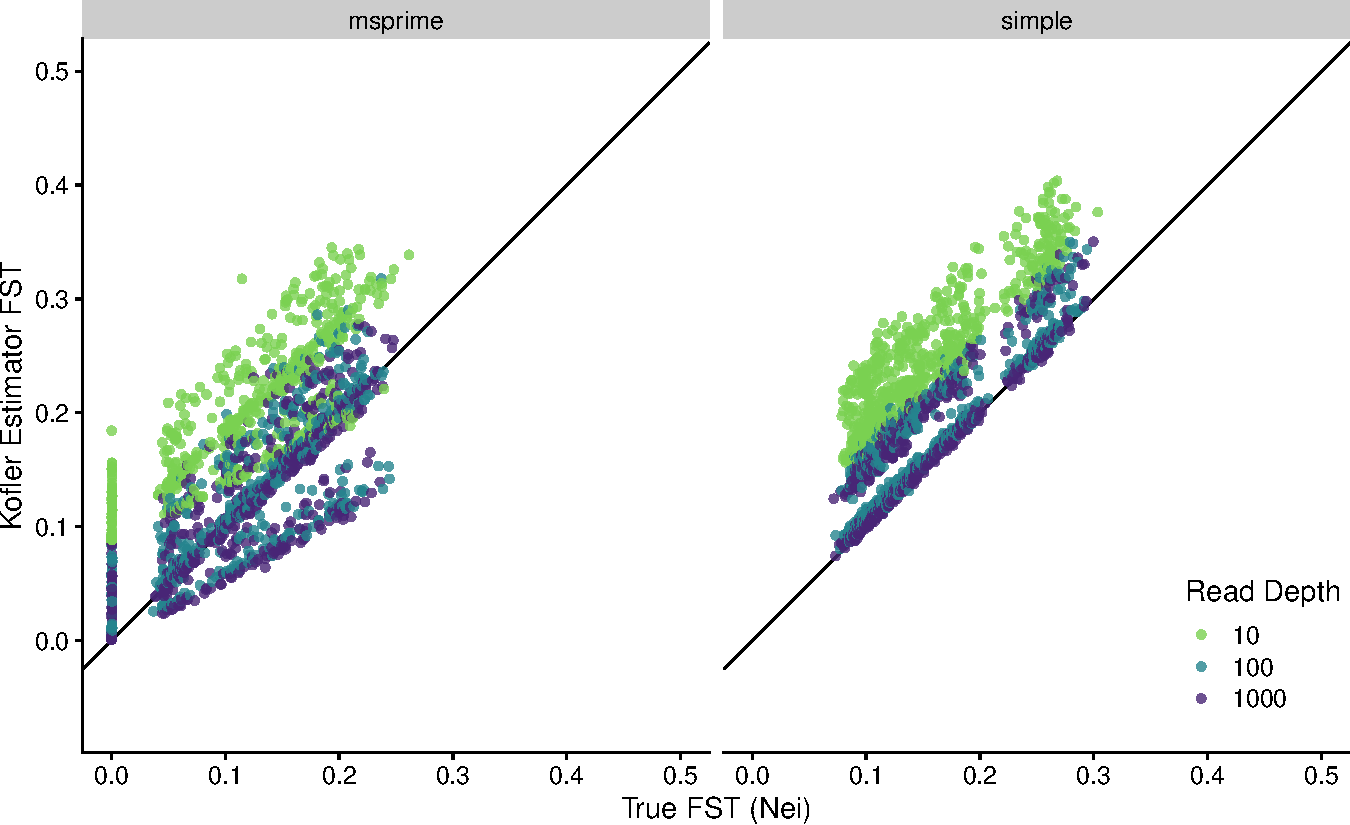
\includegraphics[width=.69\linewidth]{true_nei_fst-est_kofler-read_depth.pdf}
    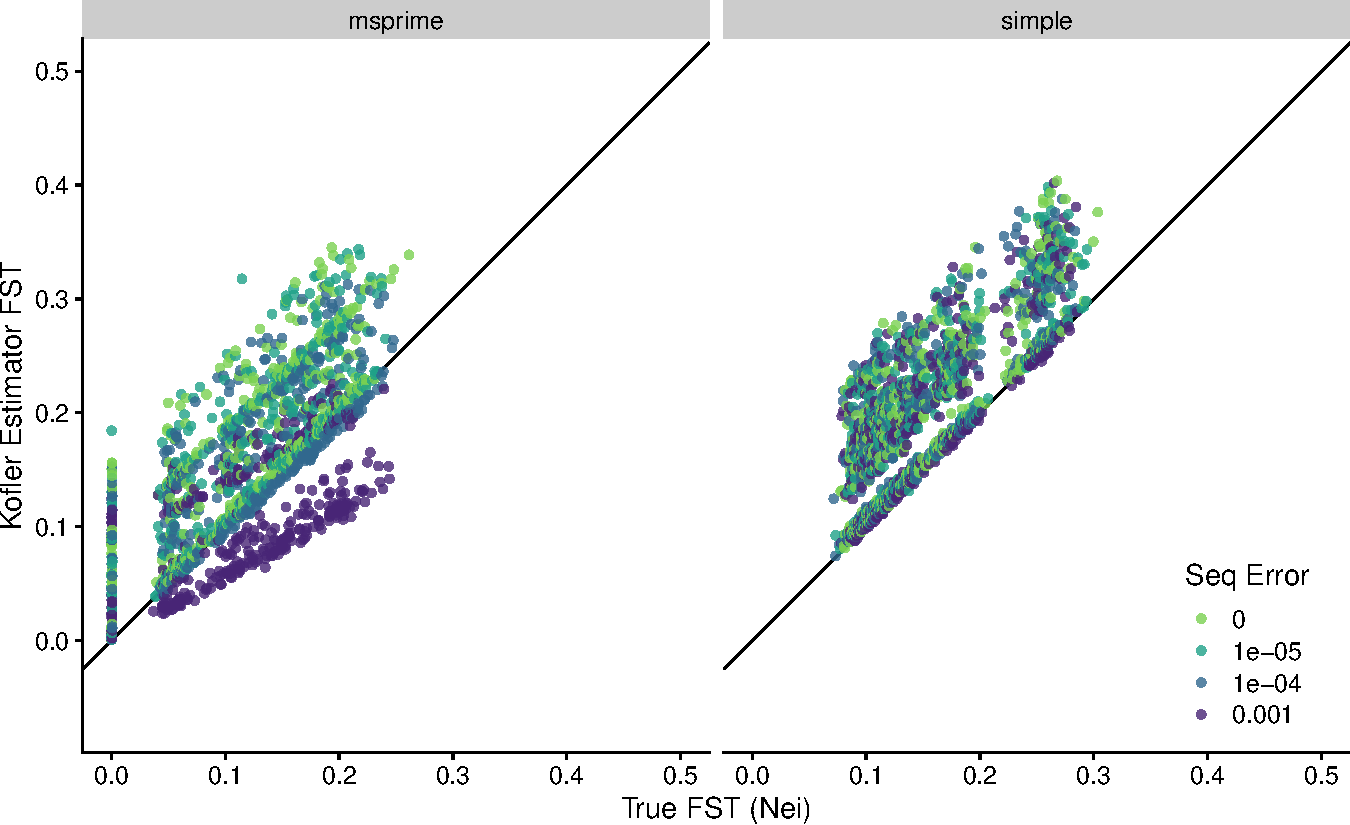
\includegraphics[width=.69\linewidth]{true_nei_fst-est_kofler-seq_error.pdf}
    \vspace*{-1em}
    \caption{
%         \textbf{Kofler}
        Kofler Estimator for FST vs true FST (Nei).
    }
\label{fig:Kofler}
\end{figure*}

\begin{figure*}[p]
    \centering
    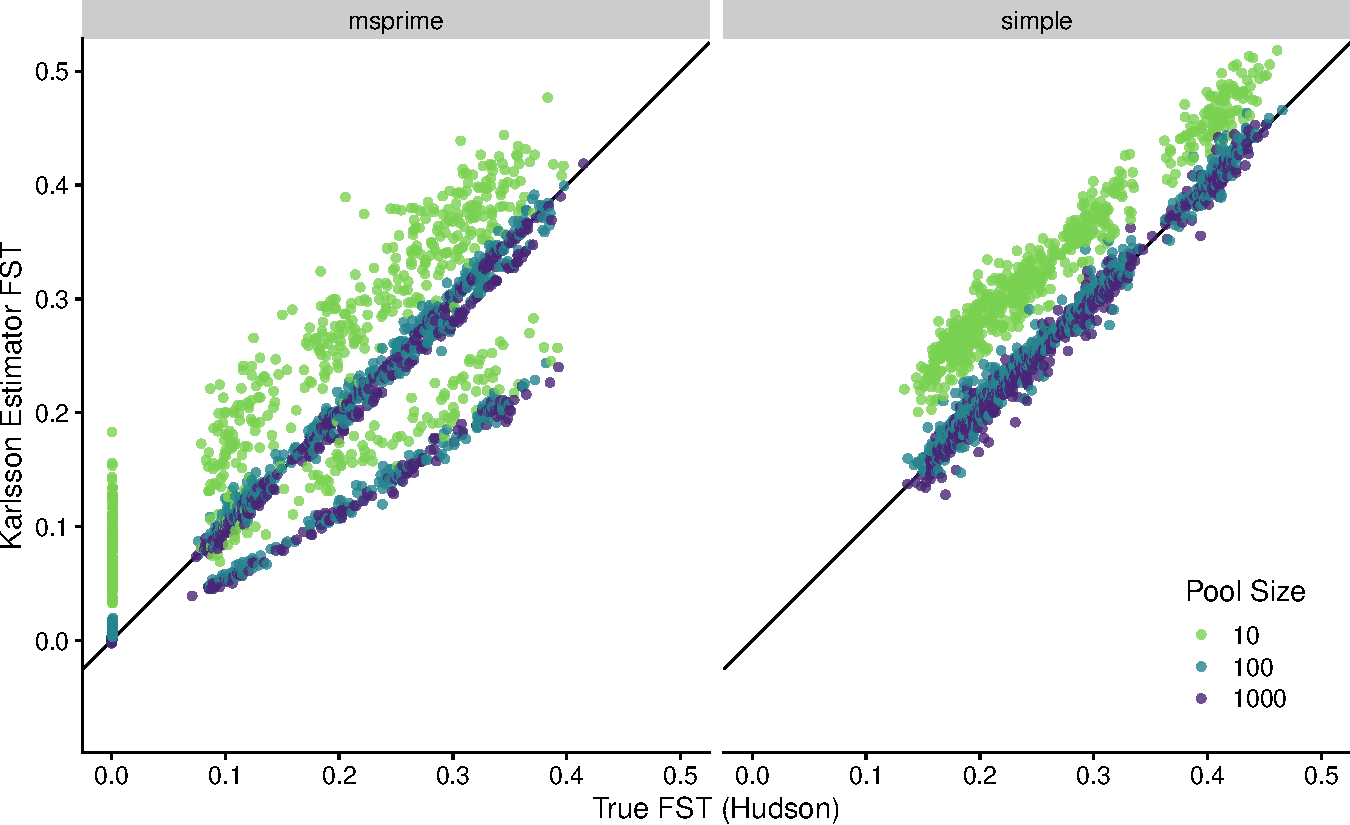
\includegraphics[width=.69\linewidth]{true_hudson_fst-est_karlsson-pool_size.pdf}
    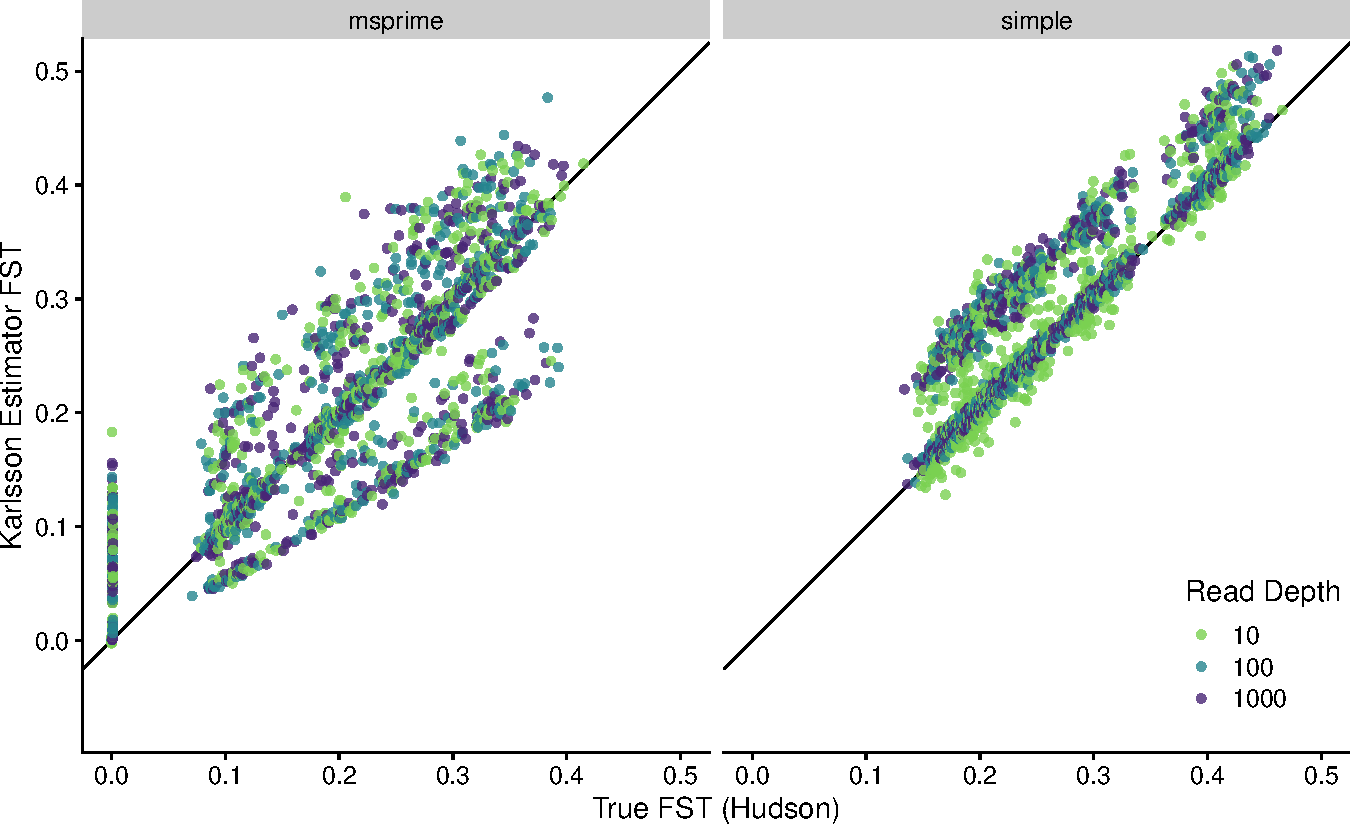
\includegraphics[width=.69\linewidth]{true_hudson_fst-est_karlsson-read_depth.pdf}
    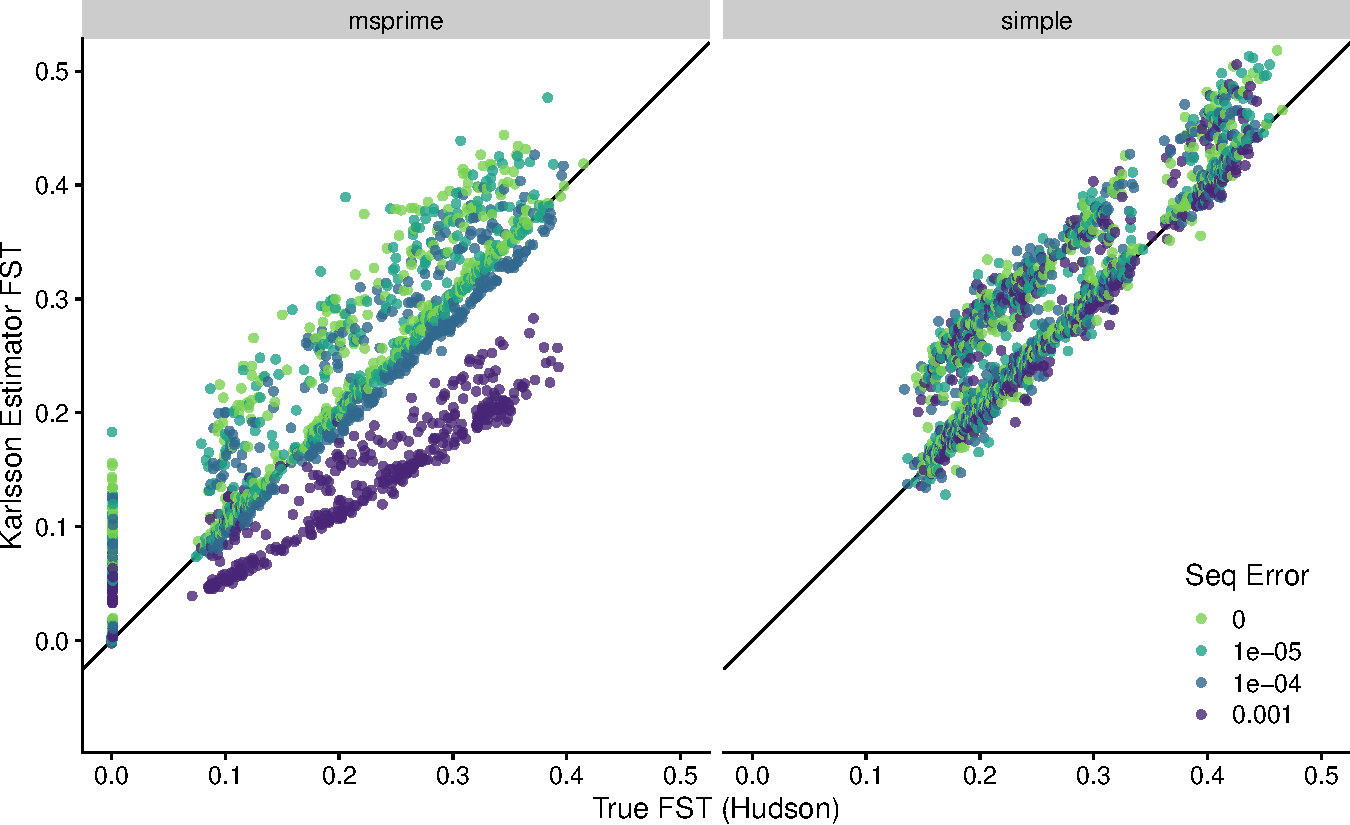
\includegraphics[width=.69\linewidth]{true_hudson_fst-est_karlsson-seq_error.pdf}
    \vspace*{-1em}
    \caption{
%         \textbf{Karlsson}
        Karlsson Estimator for FST vs true FST (Hudson).
    }
\label{fig:Karlsson}
\end{figure*}

We show the results of the simulations in Figures~\ref{fig:UnbiasedHudson}-\ref{fig:Karlsson}. Each Figure shows the comparison of the estimated values versus the true values, for \texttt{msprime} on the left, and for the "simple" simulation on the right. Each plot is repeated three times, colorized by Pool Size, Read Depth, and Sequencing Error, respectively, in order to show the effects of each of these parameters on the estimation.

We find that the estimators we derived in Section~\ref{supp:sec:FST:sub:EstimatorFST} are approximately unbiased across all regimes except for the \texttt{msprime} simulations with the highest sequencing error rate, see \figref{fig:UnbiasedHudson} and \figref{fig:UnbiasedNei}. In particular, it can be observed that for larger pool sizes, the variance of the estimators reduces, as expected, as well as, to some degree, for higher read depths.

In contrast, in \figref{fig:Kofler} we find that the Kofler estimator of $\neifst$ is highly biased in a way that depends on pool size and average read depth.  This makes sense because as discussed above, the Kofler estimate of $\pi_\text{between}$ includes a Bessel correction when it should not.  That Bessel correction contains terms that depend on both the pool size and the the read depth, explaining the pool size and sample size-dependent bias.

Similarly, in \figref{fig:Karlsson} we find that the Karlsson estimator of $\hudsonfst$ is highly biased for small pool sizes, but otherwise performs well (again except for the case of high sequencing error).  Again, this makes sense as the Karlsson estimator implicitly assumes an infinite pool size, and so will be biased for small pool sizes.

For the \texttt{msprime} simulations with the highest sequencing error rate, we see that all methods severely underestimate \fst.  It makes sense that the methods should be biased that way, as none of the estimators account for sequencing error. In the \texttt{msprime} simulations, most sites are not segregating in the population.  Sites that are not segregating do not contribute to the true value of \fst{} --- they act as a $0$ added to each of the $\pi$'s. Calling the rate of sequencing error~$\epsilon$, all of the above estimators add something $\approx \epsilon$ over the number of sites to each of the $\widehat{\pi}$'s in expectation.  As a result, for $\neiestimator := 1 - \sfrac{\widehat{\pi}_\text{within}}{\widehat{\pi}_\text{total}}$, for example, we add something on the order of $\epsilon$ to our estimates of $\widehat{\pi}_\text{within}$ and $\widehat{\pi}_\text{total}$.  This inflates $\sfrac{\widehat{\pi}_\text{within}}{\widehat{\pi}_\text{total}}$ causing us to underestimate $\neifst$.  

A similar phenomenon occurs for $\hudsonestimator$, as well as the other estimators.  To see that invariant sites add $\approx\epsilon$ over the total number of sites to any of the $\widehat{\pi}$'s, consider an asymptotic regime where both the read depth and the pool size are large.  In this regime, if there were no sequencer error, the empirical frequency of each allele across reads is a very accurate estimate of the the true population allele frequency.  In particular, for invariant sites, all of the reads will show the ``0'' allele across both populations.  If we add sequencing error, then approximately $\epsilon$ proportion of the reads will show the ``1'' allele in each population.  Our estimators as introduced above ignore sequencing error, and so in this case, it would look like both populations have the ``1'' allele at frequency $\epsilon$.  Naively plugging these frequencies into $\pi_\text{within}$, $\pi_\text{between}$, or $\pi_\text{total}$ we obtain $\epsilon(1-\epsilon)\approx \epsilon$.  In practice, at invariant sites, the different estimators would include various Bessel corrections, but the intuition holds, and these sites contribute approximately $\epsilon$ to the overall estimates of the different $\pi$'s.  As a result, if $\epsilon$ is comparable to or larger than any of the $\pi$'s, then any of the  estimators will be significantly biased.  Indeed, in the \texttt{msprime} simulations, we would expect $\pi_\text{within}$ to be approximately $\theta$, which is $0.001$, matching the highest sequencing error simulations, and explaining the apparent bias.  In contrast, in the ``simple'' simulations, $\pi_\text{within}$ is approximately $0.03$ which is an order of magnitude larger than the highest sequencing error simulated and hence the bias is negligible.

% We hence highly recommend to use our novel estimators over the ones implemented in \toolname{PoPoolation2}.

% ------------------------------------------------------------------------------------------------------
%          Unbiased estimates of heterozygosity in the presence of sequencing error
% ------------------------------------------------------------------------------------------------------
% \todo{(Moi) I think is fine to just say this and not go through equations ;) }

\subsection{Unbiased estimates of heterozygosity in the presence of sequencing error}
\label{supp:sec:FST:sub:HeterozygositySequencingError}

In the following, we present derivations of the above estimators of \fst{} that also correct for sequencing errors. This is currently not implemented in our software, and in no other software that we are aware of. Our rationale is that many applications are based on short-read Illumina sequencing, which has an error of ~1/1000. We however present it here for completeness, in the hope that this is useful for others, especially if other types of next generation sequencing with higher error rates are used.

\todo{check whether this or something similar is implemented in poolfstat! it might be important to mention this here then!}

\todo{Jeff, do you think it would be worth showing the above bias plots here again, with the seq error correction? it might mean that we have to implement the equations though... not sure if needed now. JPS: I think that sequencing error rates are high enough and pi tends to be low enough that they could actually mess up Fst estimates in practice.  People would probably appreciate a corrected estimate of Fst, but it's also probably not super crucial.  I guess it depends on how hard it is to implement. LC: it's kind of a lot to implement... instead of just keeping counts or frequencies at each position, we'd have to keep track of each base with its respective quality score throughout the whole process... a lot of code refactoring! the average one could be done more easily though, I think.}

% --------------------------------------
%     Overview
% --------------------------------------

\subsubsection*{Overview}
\label{supp:sec:FST:sub:HeterozygositySequencingError:sub:Overview}

We will derive estimators for \piw, \pib, and \pit in the presence of sequencing error.  In the simulations above, and by a hand-wavy theoretical argument, we saw that if sequencing error is on the order of \piw, \pib, or \pit, then our estimates of $F_\text{ST}$ can be severely biased.  We consider two cases: one where we have access to read-level estimates of sequencing error (e.g., phred scores), and one where we just have access to an estimate of the average sequencing error rate.  Since the second is a special case of the first (i.e., we can just assume all reads have the same sequencing error), it will follow straightforwardly but will simplify some equations.

One interesting and important observation to note here is that when we did not account for sequencing error, our estimates of \piw, \pib, and \pit were all zero for monomorphic (non-segregating) sites.  This allowed us to sum the estimates of \piw, \pib, and \pit across only segregating sites and then divide by the total number of sites (both segregating and non-segregating).  We will see that once we account for sequencing error, monomorphic sites actually contribute a small amount to \piw, \pib, and \pit, as there will now be an \emph{additive} bias correction in addition to a multiplicative one.  As such, when computing \piw, \pib, or \pit in a window, we will need to sum across segregating sites and then add a term that is the number of non-segregating sites times the estimate of \piw, \pib, or \pit for a non-segregating sites, and then finally divide that whole expression by the total number of sites.

We will start with our general model, derive our estimators from there, and then show that they are unbiased.  

% --------------------------------------
%     Model
% --------------------------------------

\subsubsection*{Model}
\label{supp:sec:FST:sub:HeterozygositySequencingError:sub:Model}

We will follow the notation from above where applicable, but briefly reintroduce some terms for ease of reading.  For generality, we will assume that there are $K$ possible alleles; this will allow us to switch between biallelic model and models on $\left\{A, C, G, T\right\}$.  We let $f_\tau$ be the frequency of allele $\tau$ \emph{in the population}.  Then we let $N_\tau$ be the (unobserved) number of individuals in the pool of $n$ individuals with allele $\tau$.  Finally, let there be $c$ reads at a site, and let $R_j$ be the allele of the individual sequenced on the $j^\text{th}$ read, and let $\hat{R}_j$ be the actual output of the sequencer for the $j^\text{th}$ read.  That is, if $R_j = \tau$, then the $j^\text{th}$ read comes from an individual that has the $\tau$ allele, but then once we sequence that fragment, there is a small chance that an error is introduced, so it is very likely that $\hat{R}_j$ --- the allele output by the sequencer --- is $\tau$ if $R_j$ is $\tau$, but there is some chance that the sequencer reads a different allele and then $\hat{R}_j = \tau' \ne \tau$.  In the most general case, we will assume that $\hat{R}_j$ matches $R_j$ with probability $1 - \epsilon_j$ and randomly chooses an allele other than $R_j$ with probability $\epsilon_j$ and chooses among the options uniformly at random.  For example, if we are looking at  $\left\{A, C, G, T\right\}$ and the sequencing error rate of read $j$ is $\epsilon_j$, then if $R_j = A$, we have that $\hat{R}_j = A$ with probability $1 - \epsilon_j$ and $\hat{R}_j = C$ with probability $\epsilon_j/3$, and $\hat{R}_j = G$ with probability $\epsilon_j/3$, and $\hat{R}_j = T$ with probability $\epsilon_j/3$.

Throughout we will use the following results for $j\ne j'$:
\begin{align}
\mathbb{E}\left[\mathbb{I}\left\{\hat{R}_j = \tau\right\}\right] &= \frac{\epsilon_j}{K-1} + \left(1 - \frac{K}{K-1} \epsilon_j\right)f_\tau \label{eq:first_moment}\\
\mathbb{E}\left[\mathbb{I}\left\{\hat{R}_j = \tau\right\}\mathbb{I}\left\{\hat{R}_{j'} = \tau\right\}\right] &= \frac{\epsilon_j\epsilon_{j'}}{(K-1)^2} \nonumber \\&\hspace{0.4cm}+ \frac{1}{n}\left((1-\epsilon_j)(1-\epsilon_{j'}) + \frac{n-1}{K-1}(\epsilon_j + \epsilon_{j'} - 2\epsilon_j\epsilon_{j'}) + \frac{1-2n}{(K-1)^2}\epsilon_j\epsilon_{j'}\right) f_\tau \label{eq:second_moment} \\&\hspace{0.4cm}+ \frac{n-1}{n}\left((1-\epsilon_j)(1-\epsilon_{j'}) - \frac{1}{K-1}(\epsilon_j + \epsilon_{j'} - 2\epsilon_j\epsilon_{j'}) + \frac{1}{(K-1)^2}\epsilon_j\epsilon_{j'})\right) f_\tau^2 \nonumber
\end{align}

Before going any further, these look a bit complex, so let's do a quick sanity check.  If $\epsilon_j = 0$, then we get
\begin{align*}
\mathbb{E}_{\epsilon=0}\left[\mathbb{I}\left\{\hat{R}_j = \tau\right\}\right] &= f_\tau\\
\mathbb{E}_{\epsilon=0}\left[\mathbb{I}\left\{\hat{R}_j = \tau\right\}\mathbb{I}\left\{\hat{R}_{j'} = \tau\right\}\right] &= \frac{1}{n}f_\tau + \frac{n-1}{n} f_\tau^2,
\end{align*}
which it turns out matches what we would get from looking at reads in the model with no error in the equations as described in the sections above.  Above, we considered the empirical frequency $\widehat{f}_\tau := \frac{1}{c}\sum_{j=1}^c \mathbb{I}\left\{\hat{R}_j = \tau\right\}$, and saw that if there is no sequencing error $\mathbb{E}\left[\widehat{f}_\tau(1-\widehat{f}_\tau)\right] = \frac{n-1}{n}\frac{c-1}{c}f_\tau(1-f_\tau)$.  We leave it as a straightforward exercise to see that the above (when all $\epsilon_j$ are zero) implies the same expectation for $\widehat{f}_\tau(1-\widehat{f}_\tau)$.

To see equation~\eqref{eq:first_moment}, note that by the tower property (twice),
\begin{align*}
\mathbb{E}\left[\mathbb{I}\left\{\hat{R}_j = \tau\right\}\right] &= \mathbb{E}\mathbb{E}\left[\mathbb{I}\left\{\hat{R}_j = \tau\right\} | R_j\right]\\
&= \mathbb{E}\left[(1-\epsilon_j) \mathbb{I}\left\{R_j = \tau \right\}\right] + \mathbb{E}\left[\frac{\epsilon_j}{K-1}\mathbb{I}\left\{R_j \ne \tau \right\}\right]\\
&= (1-\epsilon_j)\mathbb{E}\mathbb{E}\left[\mathbb{I}\left\{R_j = \tau \right\} | N_\tau \right] + \frac{\epsilon_j}{K-1}\mathbb{E}\mathbb{E}\left[\mathbb{I}\left\{R_j \ne \tau \right\} | N_\tau \right]\\
&= (1-\epsilon_j) \mathbb{E}\left[\frac{N_\tau}{n}\right] + \frac{\epsilon_j}{K-1}\mathbb{E}\left[\frac{n-N_\tau}{n}\right]\\
&= (1-\epsilon_j) f_\tau + \frac{\epsilon_j}{K-1}(1- f_\tau)\\
&= \frac{\epsilon_j}{K-1} + \left(1 - \frac{K}{K-1}\epsilon_j\right)f_\tau
\end{align*}

Equation~\eqref{eq:second_moment} follows the same reasoning but with substantially more algebra, so we omit it here for simplicity.

One last useful fact is that if we sum equations~\eqref{eq:first_moment}~and~\eqref{eq:second_moment} over $\tau$, we obtain something slightly nicer, since $\sum_\tau f_\tau =1$.  With this summation and some slight algebraic manipulation we see:
\begin{align}
\sum_{\tau}\mathbb{E}\left[\mathbb{I}\left\{\hat{R}_j = \tau\right\}\right] &= 1 \label{eq:first_moment_sum}\\
\sum_{\tau}\mathbb{E}\left[\mathbb{I}\left\{\hat{R}_j = \tau\right\}\mathbb{I}\left\{\hat{R}_{j'} = \tau\right\}\right] &= \frac{1}{n}\left((1-\epsilon_j)(1-\epsilon_{j'}) + \frac{n-1}{K-1}(\epsilon_j + \epsilon_{j'} - 2\epsilon_j\epsilon_{j'}) + \frac{(K-2)n + 1}{(K-1)^2}\epsilon_j\epsilon_{j'}\right)  \label{eq:second_moment_sum} \\&\hspace{0.4cm}+ \frac{n-1}{n}\left((1-\epsilon_j)(1-\epsilon_{j'}) - \frac{1}{K-1}(\epsilon_j + \epsilon_{j'} - 2\epsilon_j\epsilon_{j'}) + \frac{1}{(K-1)^2}\epsilon_j\epsilon_{j'})\right)  \nonumber \\ &\hspace{1cm}\times \sum_\tau f_\tau^2 \nonumber
\end{align}

With these preliminaries out of the way, we can get to our estimators.

% --------------------------------------
%     Unbiased estimator for \piw
% --------------------------------------

\subsubsection*{Unbiased estimator for \piw}
\label{supp:sec:FST:sub:HeterozygositySequencingError:sub:UnbiasedPIW}

Recall that \piw is defined as $\frac{1}{2}\left(\pi_{(1)} + \pi_{(2)}\right)$, where $\pi_{(p)}$ is the heterozygosity in population $p$.  Since this is linear, we just need an unbiased estimator for the heterozygosity within one population, and then we can average these estimators across the populations to obtain an estimator of \piw.

Our estimator is a bit unwieldy, so first we define a number of additional variables to clean up the notation.  Note that all of these only depend upon observable quantities (i.e., the sample size, coverage, and error rates) so they can be readily computed from the observed data.
\begin{align*}
\overline{\epsilon} &:= \frac{1}{c} \sum_{j=1}^c \epsilon_j\\
\overline{\epsilon^2} &:= \frac{1}{c} \sum_{j=1}^c \epsilon_j^2\\
\epsilon^* &:= (\overline{\epsilon})^2 - \frac{\overline{\epsilon^2}}{c}\\
w_1 &:= \frac{1}{c} + \frac{1}{n}\left(\frac{c-1}{c} + 2\left(\frac{c-1}{c}\right)\left(\frac{n-K}{K-1}\right)\overline{\epsilon} + \left(1 - 2\left(\frac{n-1}{K-1}\right) + \frac{(K-2)n + 1}{(K-1)^2}\right)\epsilon^*\right)\\
w_2 &:= \frac{n-1}{n}\left(\frac{c-1}{c} - 2\left(\frac{c-1}{c}\right)\left(\frac{K}{K-1}\right)\overline{\epsilon} + \left(1 + \frac{2}{K-1} + \frac{1}{(K-1)^2}\right)\epsilon^*\right)
\end{align*}

We are now ready to define our unbiased estimator of $\pi$ within a given population.  Let $\hat{f}_\tau = \sum_{j=1}^c \mathbb{I}\left\{\hat{R}_j = \tau\right\}$ be the empirical frequency of allele $\tau$ in the observed reads.
\[
\widehat{\pi} := \frac{w_1 + w_2 - \sum_\tau \hat{f}_\tau^2}{w_2}.
\]

It is a bit of work to show, but it turns out that $\mathbb{E}[\widehat{\pi}] = \pi$. Hence, this estimator is an unbiased estimator for the heterozygosity within a population.  The overall proof is to show that
\begin{align}
\sum_\tau\mathbb{E}\left[\hat{f}_\tau^2\right] &= w_1 + w_2 \sum_\tau f_\tau^2, \label{eq:lemma}
\end{align}
which we will show below, but for now we assume this being true.  Then, we can use this formula to see
\begin{align*}
\mathbb{E}\left[\widehat{\pi}\right] = \frac{w_1 + w_2 - \sum_\tau \mathbb{E}\left[\hat{f}_\tau^2\right]}{w_2} = 1 -\sum_\tau f_\tau^2 =: \pi
\end{align*}
as required.

Now to see equation~\eqref{eq:lemma}, we write
\begin{align*}
\sum_\tau\mathbb{E}\left[\hat{f}_\tau^2\right] &= \frac{1}{c^2}\sum_{j=1}^c \sum_{j'=1}^c \sum_\tau \mathbb{E}\left[\mathbb{I}\left\{\hat{R}_j=\tau\right\}\mathbb{I}\left\{\hat{R}_{j'}=\tau\right\}\right]\\
&= \frac{1}{c^2}\left\{\left(\sum_{j=1}^c \mathbb{E}\left[\mathbb{I}\left\{\hat{R}_j=\tau\right\}\right]\right) + \left( \sum_{j\ne j'}\mathbb{E}\left[\mathbb{I}\left\{\hat{R}_j=\tau\right\}\mathbb{I}\left\{\hat{R}_{j'}=\tau\right\}\right] \right) \right\}\\
&= w_1 + w_2\sum_\tau f_\tau^2
\end{align*}
where the final line follows from using Equations~\eqref{eq:first_moment_sum}~and~\eqref{eq:second_moment_sum} and then doing quite a bit of algebra.

% --------------------------------------
%     Unbiased estimator for \pib
% --------------------------------------

\subsubsection*{Unbiased estimator for \pib}
\label{supp:sec:FST:sub:HeterozygositySequencingError:sub:UnbiasedPIB}

Fortunately, the estimator for \pib is much simpler.  From equation~\eqref{eq:first_moment}, we see
\begin{align*}
\mathbb{E}\left[\hat{f}_\tau\right] &= \frac{1}{c}\sum_{j=1}^c \mathbb{E}\left[\mathbb{I}\left\{\hat{R}_j = \tau\right\}\right]\\
&= \frac{1}{c}\sum_{j=1}^c \frac{\epsilon_j}{K-1} + \left(1 - \frac{K}{K-1}\epsilon_j\right)f_\tau\\
&= \frac{\overline{\epsilon}}{K-1} + \left(1 - \frac{K}{K-1}\overline{\epsilon}\right)f_\tau
\end{align*}
Rearranging, this immediately implies that
\[
\frac{\hat{f}_\tau - \frac{\overline{\epsilon}}{K-1}}{1 - \frac{K}{K-1}\overline{\epsilon}}
\]
is unbiased for $f_\tau$.  So far we have suppressed the dependence of all of these things on the population (i.e., we've just been looking at a single sample), but for \pib we must consider two samples.  We will use a $(p)$ superscript to denote the population.  Our estimator for \pib is then
\[
\widehat{\pi}_\text{between} := 1 - \sum_\tau \left(\frac{\hat{f}^{(1)}_\tau - \frac{\overline{\epsilon}^{(1)}}{K-1}}{1 - \frac{K}{K-1}\overline{\epsilon}^{(1)}}\right)\left(\frac{\hat{f}^{(2)}_\tau - \frac{\overline{\epsilon}^{(2)}}{K-1}}{1 - \frac{K}{K-1}\overline{\epsilon}^{(2)}}\right)
\]
That this is unbiased follows immediately from the unbiasedness of our estimators of $f_\tau$ within each population and the independence of the two samples. 

% --------------------------------------
%     Unbiased estimator for \pit
% --------------------------------------

\subsubsection*{Unbiased estimator for \pit}
\label{supp:sec:FST:sub:HeterozygositySequencingError:sub:UnbiasedPIT}

Recall that $\mathpit = \frac{1}{2}\left(\mathpiw + \mathpib\right)$ so with our unbiased estimators of \piw and \pib, we immediately by the linearity of expectation obtain that:
\[
\widehat{\pi}_\text{total} := \frac{1}{2}\left(\widehat{\pi}_\text{within} + \widehat{\pi}_\text{between}\right)
\]
is unbiased for \pit.

% --------------------------------------
%     Constant error rates
% --------------------------------------

\subsubsection*{Constant error rates}
\label{supp:sec:FST:sub:HeterozygositySequencingError:sub:ConstErr}

If we assume that all reads have the same error rates, say $\epsilon$, then $\overline{\epsilon} = \epsilon$, $\overline{\epsilon^2} = \epsilon^2$, and $\epsilon^* = \frac{c-1}{c}\epsilon^2$.  Otherwise, the equations remain unchanged.


% ------------------------------------------------------------------------------------------------------
%          PoPoolation2 Equations Document
% ------------------------------------------------------------------------------------------------------
% \todo{(Moi) I think is fine to just say this and not go through equations ;) }

\section{PoPoolation Equations Document}
\label{supp:sec:PoPoolation2Equations}

The PoPoolations equation document also presents some simplifications and related equations that to the best of our knowledge are not implemented in their software.
We hence do not go through them in detail here, but still want to mention them, in case they might be useful for others.

\begin{itemize}
  \item They present simplified versions of $\theta_\pi$, $\theta_w$, and Tajima's D, which assume that allele frequency distribution in the reads is about the same as in the real population, and hence arrives at a simpler computation at the cost of some error. These are also useful for individual sequencing.
  \item As mentioned above in \secref{supp:sec:TajimaD:sub:PoolSequencingCorrection}, the document presents an approach to computing Tajima's D based on its variance, and extends this to windows, but (to the best of our knowledge) does not implement this, and instead implement their approach based on \citeay{Achaz2008}.
  \item They present an approach for computing \fst{} for $J$ pool-sequenced populations (instead of just two as presented above), extend this approach to large regions as well as single SNPs, and introduce weights that take the number of sequenced individuals in each population into account. More work is needed to compare this approach to their implementation and to our estimators.
\end{itemize}

These alternative approaches however need further assessment and comparison to the other approaches presented here.

\popoolissue{Lastly, we wanted to note that to us it seems that some equations in the PoPoolation equations document are not actually implemented in the code, and that the code contains compuations that are not in the document. We hence think that those were never intended to go hand in hand, and that hence the equations document is also not part of the official publication, but merely found in the code repository. Is that assessment correct, or are there other reasons for the divergence between the two?}

% The Pool-seq corrected equations for $\text{F}_\text{ST}$ available in the pdf document of PoPoolation's code repository are not implemented, to the best of our knowledge, in \toolname{PoPoolation} nor in \toolname{PoPoolation2} software.
% Here we describe the methods implemented in \toolname{PoPoolation2} code, explain the rationale, and expand on calculation options of our own implementation.
% See \citeay{Bhatia2013} for a good introduction to the topic and the confusion around \fst.

% The below section names are what the PoPoolation equations document offers.
% At the moment however, it seems that the implementation (which is not in \toolname{PoPoolation}, but in \toolname{PoPoolation2})
% differs from the equations that they have in their document.
% So, instead of copying the above equations from their document to here for somthing that is not even implemented,
% as of now, we leave the above blank.

% Instead, we here write down the equations that are actually implemented in \toolname{PoPoolation2}, based on the code.

% % --------------------------------------------------------
% %          Large Regions
% % --------------------------------------------------------

% \subsubsection{Large Regions}
% \label{supp:sec:FST:sub:LargeRegions}

% % --------------------------------------------------------
% %          Simplified
% % --------------------------------------------------------

% \subsubsection{Simplified Regional \texorpdfstring{\fst}{FST}}
% \label{supp:sec:FST:sub:Simplified}

% % (also good for individual sequencing again)

% % --------------------------------------------------------
% %          Single SNPs
% % --------------------------------------------------------

% \subsubsection{Single SNPs}
% \label{supp:sec:FST:sub:SingleSNPs}

% % --------------------------------------------------------
% %          Weights
% % --------------------------------------------------------

% \subsubsection{Weights}
% \label{supp:sec:FST:sub:Weights}

% % ======================================================================================================
% %          SCRATCH
% % ======================================================================================================

% \todo{the below are (commented out) reverse-engineered equations of the non-pool-seq-corrected equations that are also implemented in popoolation. we probably do not need them, but i want to keep them here for reference, if needed.}

% \section{SCRATCH}
% \label{supp:sec:SCRATCH}

% \todo{scratch space added by Lucas to write down PoPoolation equations as implemented}

% \subsection{Classical}
% \label{supp:sec:SCRATCH:sub:Classical}

% these are what popoolation calls ``classical'' computations, that is, without pool seq correction.
% they still use some equations that do not seem 100\% typical to me, but let's see.

% \textbf{classical pi:}

% \begin{align}
%     \theta_{\pi,Classical} &=  1 - \frac{2}{C(C-1)} \sum_\tau \frac{c_\tau (c_\tau - 1)}{2}
% \end{align}

% the call this computation ``average pairwise difference''.
% the 2s obviously cancel out, but i kept them here, as this is what's implemented.


% \textbf{classical theta (watterson): }

% \begin{align}
%     \theta_{W,Classical} &=  \frac{\text{\#SNPs}}{a_1(n_m)}
% \end{align}

% where $n_m$ is the median of all coverages in the given window,
% and $a_1$ again the harmonic as defined above.
% no idea if this is a thing that one does... but that's what they do.


% \textbf{classical D:}

% \begin{align}
%     D &=  \frac{\theta_{\pi,Classical} - \theta_{W,Classical}}{V}
% \end{align}

% where $V$ is called ``sqrt variance'', probably meaning square root of the variance, i.e., standard deviation?! and computed as:

% \begin{align}
%     V   &= \sqrt{ e_1 \cdot \text{\#SNPs} + e_2 \cdot \text{\#SNPs} \cdot (\text{\#SNPs} -1) } \\
%     e_1 &= \frac{ \frac{n_m + 1}{3 \cdot (n_m - 1)} - \frac{1}{a_1(n_m)} }{a_1(n_m)} \\
%     e_2 &= \frac{ \frac{2(n_m^2 + n_m + 3)}{9n_m(n_m-1)} - \frac{n_m+2}{a_1(n_m) \cdot n_m} + \frac{a_2(n_m)}{a_1(n_m)^2} }{ a_1(n_m)^2 + a_2(n_m) }
% \end{align}

% again using the median coverage $n_m$, and (squared) harmonic $a_1$ and $a_2$.


% ======================================================================================================
%          Conclusion
% ======================================================================================================

% \section{Conclusion}
% \label{supp:sec:Conclusion}

% \todo{needs updating later}

% We have here presented our current understanding of the equations and the implementation of PoPoolation \cite{Kofler2011a,Kofler2011b} for population genetic measures $\theta_\pi$, $\theta_w$, Tajima's D, and \fst{}. We have further introduced two novel estimators of \fst{} for pool-sequenced data.

% We invite everyone to join the discussion and to help establishing well-founded theory of these measures for pool sequencing.
% Hence, this document is a draft, and more work is needed to thoroughly assess the whole situation.
% % There might be bugs in the \toolname{PoPoolation} implementation of Tajima's D.


% ######################################################################################################################
%         Appendices
% ######################################################################################################################

% \clearpage

% Bibliography
% \bibliographystyle{pnas-new}
\bibliographystyle{natbib}
% \bibliographystyle{apalike}
% \bibliographystyle{myabbrvnat}

\bibliography{references}

\end{document}
